%%%%%%%%%%%%%%%%%%%%%%%%%%%%%%%%%%%%%%%%%
% Masters/Doctoral Thesis 
% LaTeX Template
% Version 1.43 (17/5/14)
%
% This template has been downloaded from:
% http://www.LaTeXTemplates.com
%
% Original authors:
% Steven Gunn 
% http://users.ecs.soton.ac.uk/srg/softwaretools/document/templates/
% and
% Sunil Patel
% http://www.sunilpatel.co.uk/thesis-template/
%
% License:
% CC BY-NC-SA 3.0 (http://creativecommons.org/licenses/by-nc-sa/3.0/)
%
% Note:
% Make sure to edit document variables in the Thesis.cls file
%
%%%%%%%%%%%%%%%%%%%%%%%%%%%%%%%%%%%%%%%%%

%----------------------------------------------------------------------------------------
%	PACKAGES AND OTHER DOCUMENT CONFIGURATIONS
%----------------------------------------------------------------------------------------

\documentclass[11pt, oneside]{Thesis} % The default font size and one-sided printing (no margin offsets)

\graphicspath{{Pictures/}} % Specifies the directory where pictures are stored

\usepackage[square, numbers, comma, sort&compress]{natbib} % Use the natbib reference package - read up on this to edit the reference style; if you want text (e.g. Smith et al., 2012) for the in-text references (instead of numbers), remove 'numbers' 
\hypersetup{urlcolor=blue, colorlinks=true} % Colors hyperlinks in blue - change to black if annoying
\title{\ttitle} % Defines the thesis title - don't touch this

\begin{document}
	
\frontmatter % Use roman page numbering style (i, ii, iii, iv...) for the pre-content pages

\setstretch{1.3} % Line spacing of 1.3

% Define the page headers using the FancyHdr package and set up for one-sided printing
\fancyhead{} % Clears all page headers and footers
\rhead{\thepage} % Sets the right side header to show the page number
\lhead{} % Clears the left side page header

\pagestyle{fancy} % Finally, use the "fancy" page style to implement the FancyHdr headers

\newcommand{\HRule}{\rule{\linewidth}{0.5mm}} % New command to make the lines in the title page

% PDF meta-data
\hypersetup{pdftitle={\ttitle}}
\hypersetup{pdfsubject=\subjectname}
\hypersetup{pdfauthor=\authornames}
\hypersetup{pdfkeywords=\keywordnames}

%----------------------------------------------------------------------------------------
%	TITLE PAGE
%----------------------------------------------------------------------------------------

\begin{titlepage}
\begin{center}

\textsc{\LARGE \univname}\\[1.5cm] % University name
\textsc{\Large Master's Thesis}\\[0.5cm] % Thesis type

\HRule \\[0.4cm] % Horizontal line
{\huge \bfseries \ttitle}\\[0.4cm] % Thesis title
\HRule \\[1.5cm] % Horizontal line
 
\begin{minipage}{0.4\textwidth}
\begin{flushleft} \large
\emph{Author:}\\
\authornames % Author name - remove the \href bracket to remove the link
\end{flushleft}
\end{minipage}
\begin{minipage}{0.4\textwidth}
\begin{flushright} \large
\emph{Supervisors:} \\
\supname \\ % Supervisor name - remove the \href bracket to remove the link  
\examname
\end{flushright}
\end{minipage}\\[3cm]
 
\large \textit{A thesis submitted in fulfilment of the requirements\\ for the degree of \degreename}\\[0.3cm] % University requirement text
\textit{in the course}\\[0.4cm]
\deptname\\[2cm] % Research group name and department name
 
{\large March 17\textsuperscript{th}, 2023}\\[4cm] % Date
%\includegraphics{Logo} % University/department logo - uncomment to place it
 
\vfill
\end{center}

\end{titlepage}

%----------------------------------------------------------------------------------------
%	DECLARATION PAGE
%	Your institution may give you a different text to place here
%----------------------------------------------------------------------------------------

\Declaration{

\addtocontents{toc}{\vspace{1em}} % Add a gap in the Contents, for aesthetics

I, \authornames, declare that this thesis titled, '\ttitle' and the work presented in it are my own. I confirm that:

\begin{itemize} 
\item[\tiny{$\blacksquare$}] This work was done wholly or mainly while in candidature for a research degree at this University.
\item[\tiny{$\blacksquare$}] Where any part of this thesis has previously been submitted for a degree or any other qualification at this University or any other institution, this has been clearly stated.
\item[\tiny{$\blacksquare$}] Where I have consulted the published work of others, this is always clearly attributed.
\item[\tiny{$\blacksquare$}] Where I have quoted from the work of others, the source is always given. With the exception of such quotations, this thesis is entirely my own work.
\item[\tiny{$\blacksquare$}] I have acknowledged all main sources of help.
\item[\tiny{$\blacksquare$}] Where the thesis is based on work done by myself jointly with others, I have made clear exactly what was done by others and what I have contributed myself.\\
\end{itemize}
 
Signed:\\
\rule[1em]{25em}{0.5pt} % This prints a line for the signature
 
Date:\\
\rule[1em]{25em}{0.5pt} % This prints a line to write the date
}

\clearpage % Start a new page

%----------------------------------------------------------------------------------------
%	QUOTATION PAGE
%----------------------------------------------------------------------------------------

\pagestyle{empty} % No headers or footers for the following pages

\null\vfill % Add some space to move the quote down the page a bit

\textit{``Thanks to my solid academic training, today I can write hundreds of words on virtually any topic without possessing a shred of information, which is how I got a good job in journalism."}

\begin{flushright}
Dave Barry
\end{flushright}

\vfill\vfill\vfill\vfill\vfill\vfill\null % Add some space at the bottom to position the quote just right

\clearpage % Start a new page

%----------------------------------------------------------------------------------------
%	ABSTRACT PAGE
%----------------------------------------------------------------------------------------

\addtotoc{Abstract} % Add the "Abstract" page entry to the Contents

\abstract{\addtocontents{toc}{\vspace{1em}} % Add a gap in the Contents, for aesthetics

The Thesis Abstract is written here (and usually kept to just this page). The page is kept centered vertically so can expand into the blank space above the title too\ldots
}

\clearpage % Start a new page

%----------------------------------------------------------------------------------------
%	ACKNOWLEDGEMENTS
%----------------------------------------------------------------------------------------

\setstretch{1.3} % Reset the line-spacing to 1.3 for body text (if it has changed)

\acknowledgements{\addtocontents{toc}{\vspace{1em}} % Add a gap in the Contents, for aesthetics

The acknowledgements and the people to thank go here, don't forget to include your project advisor\ldots
}
\clearpage % Start a new page

%----------------------------------------------------------------------------------------
%	LIST OF CONTENTS/FIGURES/TABLES PAGES
%----------------------------------------------------------------------------------------

\pagestyle{fancy} % The page style headers have been "empty" all this time, now use the "fancy" headers as defined before to bring them back

\lhead{\emph{Contents}} % Set the left side page header to "Contents"
\tableofcontents % Write out the Table of Contents

\lhead{\emph{List of Figures}} % Set the left side page header to "List of Figures"
\listoffigures % Write out the List of Figures

\lhead{\emph{List of Tables}} % Set the left side page header to "List of Tables"
\listoftables % Write out the List of Tables

%----------------------------------------------------------------------------------------
%	ABBREVIATIONS
%----------------------------------------------------------------------------------------

\clearpage % Start a new page

\setstretch{1.5} % Set the line spacing to 1.5, this makes the following tables easier to read

\lhead{\emph{Abbreviations}} % Set the left side page header to "Abbreviations"
\listofsymbols{ll} % Include a list of Abbreviations (a table of two columns)
{
\textbf{LAH} & \textbf{L}ist \textbf{A}bbreviations \textbf{H}ere \\
%\textbf{Acronym} & \textbf{W}hat (it) \textbf{S}tands \textbf{F}or \\
}

%----------------------------------------------------------------------------------------
%	PHYSICAL CONSTANTS/OTHER DEFINITIONS
%----------------------------------------------------------------------------------------
%
%\clearpage % Start a new page
%
%\lhead{\emph{Physical Constants}} % Set the left side page header to "Physical Constants"
%
%\listofconstants{lrcl} % Include a list of Physical Constants (a four column table)
%{
%Speed of Light & $c$ & $=$ & $2.997\ 924\ 58\times10^{8}\ \mbox{ms}^{-\mbox{s}}$ (exact)\\
% Constant Name & Symbol & = & Constant Value (with units) \\
%}

%----------------------------------------------------------------------------------------
%	SYMBOLS
%----------------------------------------------------------------------------------------
%
%\clearpage % Start a new page
%
%\lhead{\emph{Symbols}} % Set the left side page header to "Symbols"
%
%\listofnomenclature{lll} % Include a list of Symbols (a three column table)
%{
%$a$ & distance & m \\
%$P$ & power & W (Js$^{-1}$) \\
% % Symbol & Name & Unit \\
%
%& & \\ % Gap to separate the Roman symbols from the Greek
%
%$\omega$ & angular frequency & rads$^{-1}$ \\
% Symbol & Name & Unit \\
%}


%----------------------------------------------------------------------------------------
%	DEDICATION
%----------------------------------------------------------------------------------------
%
%\setstretch{1.3} % Return the line spacing back to 1.3
%
%\pagestyle{empty} % Page style needs to be empty for this page
%
%\dedicatory{For/Dedicated to/To my\ldots} % Dedication text
%
%\addtocontents{toc}{\vspace{2em}} % Add a gap in the Contents, for aesthetics
%


%----------------------------------------------------------------------------------------
%	THESIS CONTENT - CHAPTERS
%----------------------------------------------------------------------------------------

\mainmatter % Begin numeric (1,2,3...) page numbering

\pagestyle{fancy} % Return the page headers back to the "fancy" style

% Include the chapters of the thesis as separate files from the Chapters folder
% Uncomment the lines as you write the chapters

% !TeX spellcheck = en_US

% ==== Containerized multi-level deployment for a distributed adaptive microservice application ====

% Chapter 1

\chapter{Introduction} % Main chapter title

\label{chap:introd} % For referencing the chapter elsewhere, use \ref{Chapter1} 

\lhead{Chapter  \ref*{chap:introd}. \emph{Introduction}} % This is for the header on each page - perhaps a shortened title


The containerization of applications became more and more popular in the recent decade. Running applications in an isolated environment makes them more easy to manage and easier to deploy. The lightweight method of isolating processes is the basis for deploying applications on a cluster environment.
Deployed applications on distributed systems can nowadays profit from more reliability and availability. Additionally, the services can gain a higher performance due to horizontal scaling mechanisms. This means, instead of increasing performance by upgrading the hardware, the services are accessible on multiple servers.
By having a microservice architecture, complex systems are well prepared for a distributed system. The several services of the application are responsible for just their own task and thus can be scaled horizontally.

This thesis explores the feasibility of deploying a \ac{Windows} based microservice application on a cluster and gives an overview about the faced challenges. The feasibility is showcased on the basis of \ac{OT}. \ac{OT} is a distributed application for computer aided design and physics simulation. The application is distributed, thus computations can be done server-side, while the operation by the user stays client-side.
Accordingly, the orchestration has to take the multi-level architecture into account. This means that some services should only accessible in a private network space and do not require a public \ac{IP} address, while others have to be publicly available. Further, the communication has to be achieved bidirectional. Considering that clients are often protected by a firewall and located behind \ac{NAT}, this is another challenge to face.
Additionally, the architecture of \ac{OT} is adaptive by automatically spawning new processes where they are needed. Hence the application is performing an implicit load balancing based on the system resources.
Because security requirements have to be met, the network communication of \ac{OT} is encrypted with mutual authentication. Using the two-sided encryption ensures authenticity on both sides, the client and the server. The deployment has to take this into account, by distributing and creating certificates for each service and sharing them across the cluster.

The majority of deployments is still performed on Linux, even though applications orchestration for \ac{Windows} is gaining more and more demand. Recently Microsoft introduced with \enquote{Windows Containers} its own container technology\cite{Microsoft.2022}. Since the common orchestration \acf{K8s} dropped the support for Docker containers, the requested container technology on \ac{Windows} shifted towards Windows Containers\cite{Kubernetes.2020}.
\ac{OT} is based on \ac{Windows}, and thus the orchestration and containerization has to be aligned towards Windows Containers. Hence this is a fundamental task of this thesis.

Because of the recent change in isolation techniques, the previous research in this field is sparse. The documentations and guides are mostly based on the containerization using Docker and do not take the problems of the native container technology into account. 
Thus, the thesis aims to provide a valuable resource for research groups and developers who want to deploy applications using the modern Windows Container technology.

Another aspect is the introduction of a cluster using \ac{Windows} as compute nodes. Finding an orchestration engine with full support for \ac{Windows} is difficult. As shown in this thesis, \ac{K8s} as chosen orchestration engine also has struggles adding \ac{Windows} nodes into the cluster.

\begin{comment}
Nevertheless, the benefits come with the price of required application changes and higher system requirements.

Because 
Microservice applications consist of multiple services where each service fulfills its specific task. They meet the requirements for 


Applications that are served on a cluster need to fulfill the corresponding architecture requirements for a cluster environment.  and they 

This thesis explores the design and development of an cluster for an microservice application.
With regards to the automation of steps.

The requirements for serving applications in a cluster are the underlying

 the dependency on external services is high. 

The application under study, \acf{OT}, is well prepared for a cluster deployment.

\ac{K8s} was mainly used on Linux systems in the past

 there is a growing need to deploy microservice applications on Windows platforms as well. 

The thesis examines the challenges involved in deploying such an application on Windows


The research field of cluster deployment with ContainerD is still in the beginning state for \ac{Windows}.
\end{comment}


% TODO: Wenig vorarbeiten
% TODO: Multi-layer to explain




The next chapter (\autoref{chap:background}) of the thesis provides a brief introduction into \ac{OT} and its architecture. Furthermore, it introduces its encryption protocol and gives an outline about the overall topic. In \autoref{chap:design}, the major design decisions are explained. It dives into the used container engine and the chosen cluster management software and their alternatives.
The design decisions are implemented in \autoref{chap:implementation}. This is where the application is adapted by the required changes. The application is containerized, and the cluster is set up. Moreover, the probed options for designing the cluster are presented and the deployment of an application is shown.
The findings are discussed in \autoref{chap:results}. A deeper look is taken in challenges that occurred during the implementation and the underlying reasons.
The thesis ends with \autoref{chap:conclusion} and gives an overview about the conclusion and future work.

% !TeX spellcheck = en_US
% Chapter Template

\chapter{Background and problem statement} % Main chapter title

\label{chap:background} % Change X to a consecutive number; for referencing this chapter elsewhere, use \ref{ChapterX}

\lhead{Chapter \ref*{chap:background}. \emph{Background and problem statement}} % Change X to a consecutive number; this is for the header on each page - perhaps a shortened title

\section{Application under study}
\acf{OT} is a open-source simulation platform developed by the university of Applied Sciences in Frankfurt, Germany. It covers features like computer aided design and meshing and is also a physics simulation (having solvers for Finite Integration and PHREEC). The projects can be administered by a user and group management (see~\autoref{fig:ot-project}). Furthermore, all changes on a project are version-controlled. The application is designed in a way, that only a local thin-client needs to run on the users computer. After entering the login credentials (see~\autoref{fig:ot-login}), the client securely connects to a centralized service platform where the computation is made. The results and even the \ac{UI} information is sent back to the client application. This has the benefit, that also weak computers can run the application.

\begin{figure}[ht]
	\centering
	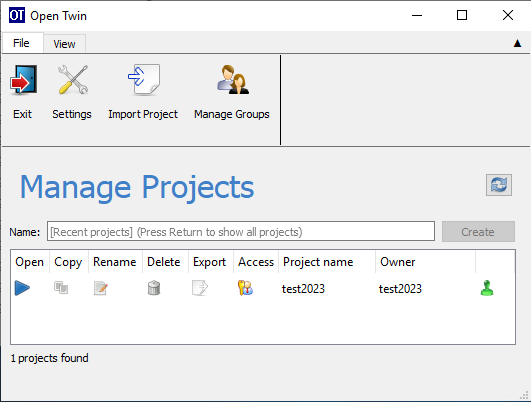
\includegraphics[width=.9\textwidth]{Figures/ot-project.png}
	\caption{The \ac{OT} project overview.}
	\label{fig:ot-project}
\end{figure}

\begin{figure}[ht]
	\centering
	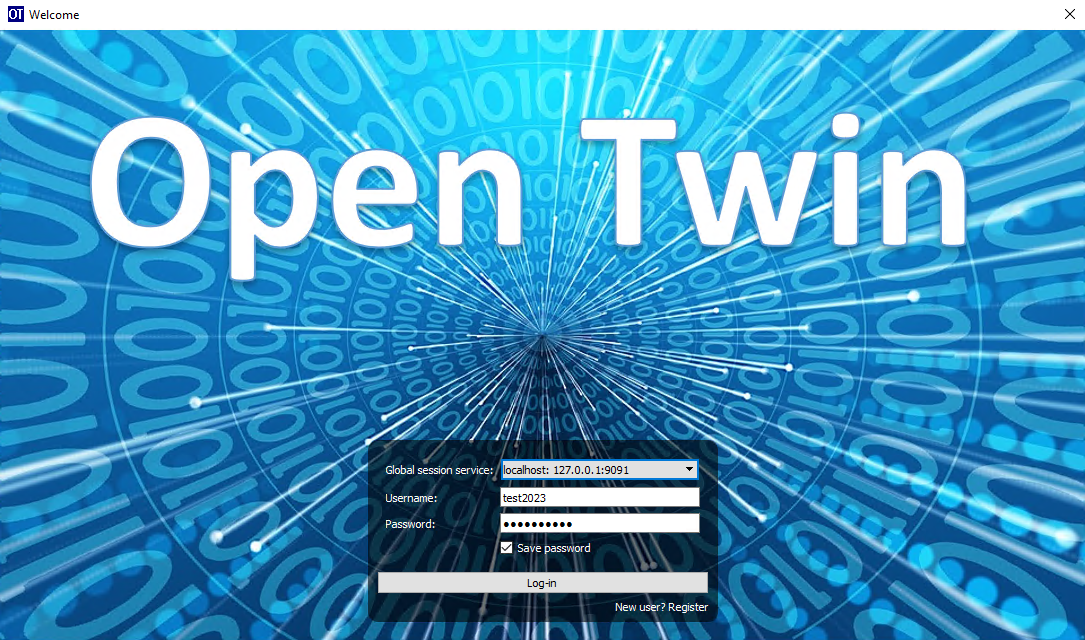
\includegraphics[width=.9\textwidth]{Figures/ot-login.png}
	\caption{The \ac{OT} login screen.}
	\label{fig:ot-login}
\end{figure}

\autoref{fig:ot-model} shows the application itself with a loaded project and a simple geometric model.
\begin{figure}[ht]
	\centering
	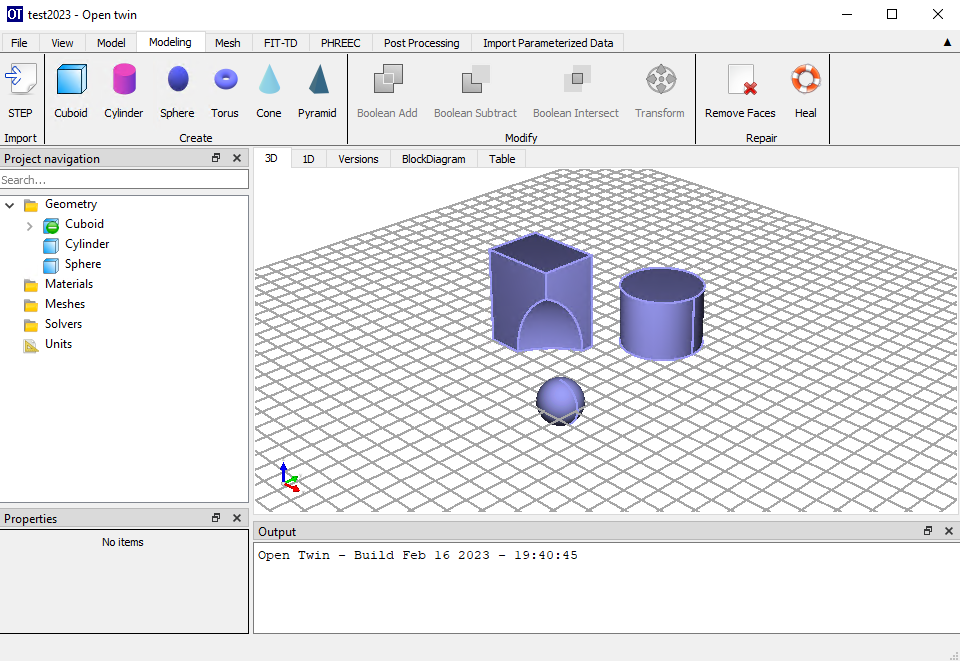
\includegraphics[width=.9\textwidth]{Figures/ot-model.png}
	\caption{A opened project inside \ac{OT} with a few created geometric models and subtracted computation.}
	\label{fig:ot-model}
\end{figure}

The development team consists of a small core team and several student groups during the semester.


\section{Baseline architecture}
\label{chap:background.baseline_architecture}
The current system design consists of multiple levels. It is a multi-process application based on the programming languages C++ and Rust. The source code is mainly aligned to be built on Microsoft \ac{Windows}. A port to Unix based systems is currently in work. Therefore parts of the code base are aligned for multiple system architectures already, but the application is not yet able to be compiled for Linux.

Each microservice of the application is included dynamically and linked as a \ac{DLL} file. For starting the microservice environment, a central executable (\enquote{open\_\ twin.exe}) is started with the corresponding arguments for the services (like the server's binding address, port numbers, and passwords) (see~\autoref{lst:ot-command}) and the path to the \ac{DLL} file itself. The UI front end, which is started by the user directly, is compiled in its own executable (\enquote{uiFrontend.exe}).

\begin{lstlisting}[language=sh, caption={Command line of Open Twin Service start}, label=lst:ot-command]
open_twin.exe GlobalSessionService.dll \
  "0" "127.0.0.1:8091" "tls@127.0.0.1:27017" "127.0.0.1:8092"
\end{lstlisting}

For conveniently running the services with all their necessary arguments, batch files were provided that read environment variables and convert them into runtime arguments for the service executable. Therefore, if the services are started locally, the user runs a batch file that sets up the environment for the network binding details, path to certificates and encrypted database credentials.

The system consists of the following micro services that are permanently accessible: \acf{GSS}, \acf{AUTH} and the database. The database is running on MongoDB\footnote{MongoDB:~https://www.mongodb.com/}. Another Service is the \acf{LSS} that spawns the so called compute services. Those are services for running the actual computation after opening a project that can dynamically spawn and exit. A partial list of compute services and their corresponding tasks can be found in \autoref{tbl:ot-compute-services}.
Each service runs in its own \ac{OS} process.

\begin{table}[h!]
	\centering
	\begin{tabular}{|l | p{.65\textwidth}|} 
		\hline
		\bfseries Name & \bfseries Task  \rule{-5pt}{2.6ex} \\
		\hline \rule{-3pt}{3ex}
		CartesianMeshService & If demanded, it converts a continuous geometry into a discrete Cartesian mesh. \\
		FITTDService & If demanded, it runs a solver algorithm for transle electromagnetic simulation based on the finite integration technique (FIT).\\
		KrigingService & If demanded, it runs a kriging interpolation of result data. \\ 
		LoggerService & A background service, that accepts logging messages from other services. \\ 
		ModelingService & Performs calculations for the creation, modeling and boolean combination of geometric data. \\ 
		PHREECService & If demanded, it runs simulation based on PHREEC. \\ 
		TetMeshService & If demanded, it meshes a form with an tetrahedral mesh.  \\ 
		VisualizationService & Runs the graphical calculations for displaying the geometric and data based results on the \ac{UI}.\\ 
		[1ex] 
		\hline
	\end{tabular}
	\caption{List of compute services and their corresponding tasks.}
	\label{tbl:ot-compute-services}
\end{table}

The Visualization Service requires features from version 2.0 of the graphics library OpenGL\footnote{OpenGL: https://opengl.org/}. Systems where no graphics card is installed or systems that run a server \ac{OS} do not have OpenGL 2.0 available. For these environments the \ac{DLL} file \enquote{opengl32sw.dll} in the installation directory can be renamed to \enquote{opengl32.dll}. This enables software rendering and allows system to run \ac{OT} that do not meet this requirement.

As shown in \autoref{fig:ot-network-communication-diagram}, the services can be separated by their network space on multiple layers. Not all services require a public available network address.
While \ac{GSS}, \ac{AUTH} and database are globally accessible via a fixed network address, the \ac{LSS} can theoretically run on a dedicated host and is only communicated to other parties after it has registered itself to the \ac{GSS}. The services, spawned by \ac{LSS} do not require a public address space either. All communication between the \ac{UI} front end and the compute services is achieved via a relay service and a web socket communication channel.

\begin{figure}[ht]
	\centering
	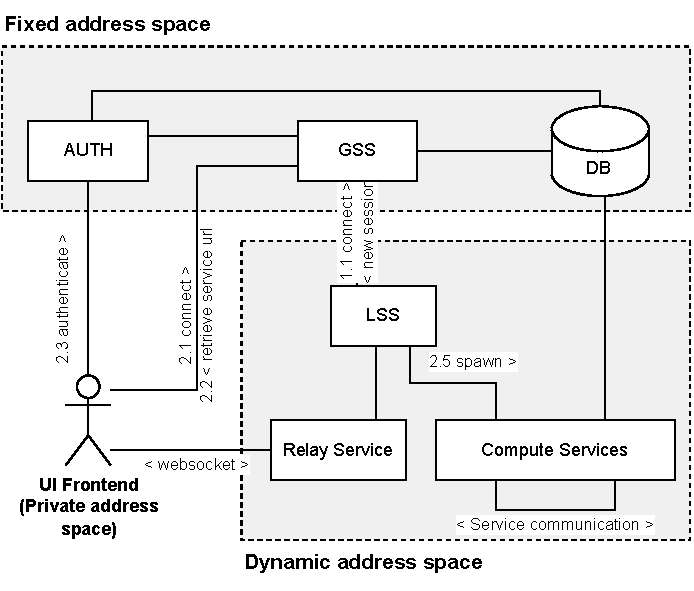
\includegraphics[width=0.8\textwidth]{Figures/opentwin-network-communication-diagram.pdf}
	\caption{Communication overview and service organization for \ac{OT} main services. In 1.1 the \ac{LSS} registers at \ac{GSS}. As soon as the \ac{UI} front end connects to the \ac{GSS}~(2.1), service information is exchanged~(2.2) and the user is authenticated~(2.3). As a consequence, the \ac{GSS} creates a new session and tells the \ac{LSS} to spawn new compute services. From now on the \ac{UI} front end communicates directly with the Compute services via the Relay Service over a web socket connection.}
	\label{fig:ot-network-communication-diagram}
\end{figure}


The whole process of the \ac{LSS} registration and connection of the \ac{UI} front end to the compute services is depicted in \autoref{fig:ot-network-communication-sequence}.
Once started, the user can login. In order to connect to the database, the following steps are performed:
\begin{enumerate}
\item The \ac{UI} front end requests further service information from the publicly available \ac{GSS}. The address for this service is provided by the user. The \ac{GSS} responds with \acp{URL} to the database and the \ac{AUTH}.
\item The \ac{UI} front end connects to the \ac{AUTH} using the authentication information provided by the user.
\item If the \ac{AUTH} replies with a positive authentication, the \ac{UI} front end connects to the database and lists the projects.
\item Once a project is opened or created, the \ac{UI} front end requests a new session from the \ac{GSS}. The \ac{GSS} replies with the connection \acp{URL} of the \ac{LSS}. The \ac{LSS} has been registered to the \ac{GSS} during its initialization.
\item The \ac{UI} front end then connects to the \ac{LSS} and requests a new session. As a result, the \ac{LSS} spawns new application service processes and replies with the respective service \acp{URL}.
\item From now on, the \ac{UI} front end communicates with the application services via the Relay service over a web socket.
\end{enumerate}

\begin{figure}[ht]
	\centering
	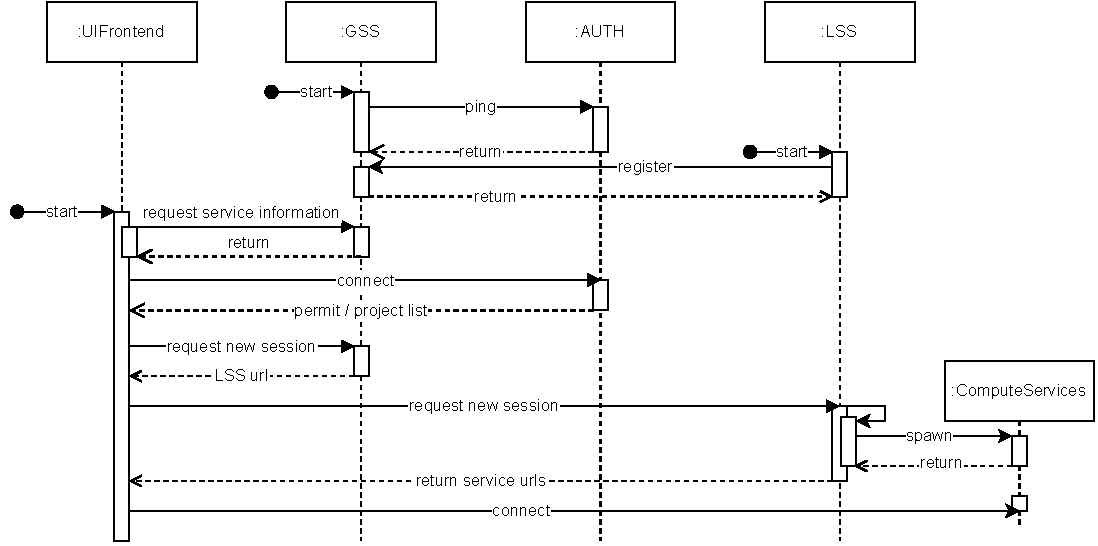
\includegraphics[width=0.99\textwidth]{Figures/opentwin-network-communication-sequence.pdf}
	\caption{Service initialization of \ac{OT} processes. In the beginning, the main services \ac{GSS}, \ac{AUTH} and an optional \ac{LSS} are initialized. While the \ac{GSS} checks the reachability of \ac{AUTH}, the \ac{LSS} registers itself at the \ac{GSS}. After starting the \ac{UI} front end, the service information is requested from a \ac{GSS} and the user is authenticated. Afterwards, the project list for the authenticated user is displayed. After opening a project, the \ac{UI} front end connects to the \ac{LSS} and requests a new session. As consequence, the \ac{LSS} spawns the compute services and connects them to the \ac{UI} front end via a Relay Service. (Ping messages are omitted.)}
	\label{fig:ot-network-communication-sequence}
\end{figure}

%The traffic between services is encrypted using \ac{mTLS} technology. While regular \ac{TLS} ensures the authenticity of the server by using Certificates and the chain of trust, it does not verify the identity of the client. This is the benefit of \ac{mTLS}. In \ac{mTLS}, both sides, client and server has to verify their identity by providing a certificate inherited from a common root authority.


\section{Network traffic encryption}

Each service of \ac{OT} offers two different channels for secure communication between services. One channel supports traditional one-way \ac{TLS}, while the other uses bidirectional \ac{mTLS}. The one-way \ac{TLS} channel is mostly used for checking the general health state of a service, while the two-way \ac{mTLS} is used for relevant application based communication.
In this section both encryption methods are briefly presented.

\subsection{Transport Layer Security}
\ac{TLS} is an cryptography extension mainly designed for providing security over \ac{HTTP}. The main goals of cryptography are confidentiality, integrity and authenticity between two communicating parties. This means, the communication on a network is kept secret between the two endpoints (Confidentiality), messages are not subject of manipulation (Integrity), and message exchanges are only allowed between authorized and trusted individuals (Authenticity). \ac{TLS} ensures the three traits by using certificates.

A simplified handshake of the \ac{TLS} protocol is depicted in \autoref{fig:tls-protocol}.
After sending the certificate from server to the client, the client validates the certificate based on the chain of trust. This means, it checks if the certificate was issued by a trusted root authority (so called \ac{CA}). Only if the authenticity of the server is ensured, the encryption key is exchanged in order to start an encrypted communication.

\begin{figure}[ht]
	\centering
	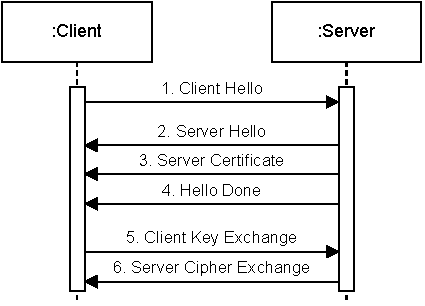
\includegraphics[width=0.6\textwidth]{Figures/tls.pdf}
	\caption{Simplified visualization of the \ac{TLS} handshake\cite{Rescorla.2018}. After initialization of the handshake (1,2), the server sends its certificate (3) and finishes with a message \enquote{Hello Done} (4). The client then validates the certificate and compares it against the chain of trust. Afterwards, the key exchange starts (5,6) to ensure an encrypted communication.}
	\label{fig:tls-protocol}
\end{figure}


\subsection{Mutual authentication}
The mutual authentication is adding another step to the one-way authentication. The application of it is used in \ac{mTLS} as extension of the classic \ac{TLS} protocol\cite{Rescorla.2018, HugoKrawczyk.2016}. Instead of just sending the server's certificate to the client, the client also sends a certificate to the server. Therefore, not only the authenticity of the server is ensured, but also of the client.

As can be seen in \autoref{fig:mtls-protocol}, compared to the \ac{TLS} handshake, the \ac{mTLS} handshake involves additional messages 5 and 6 for sending and validating the client's certificate.
Unlike with the server certificate, the client certificate is not validated against a publicly available root authority\cite{Cloudflare.20230309, Rescorla.2018}. Instead, the server acts as root authority, creates the client certificate and ships it with the application\cite{Cloudflare.20230309}.


\begin{figure}[ht]
	\centering
	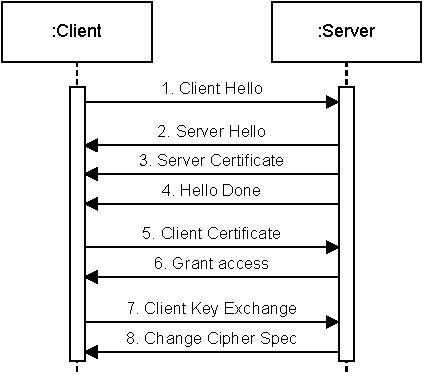
\includegraphics[width=0.6\textwidth]{Figures/mtls.pdf}
	\caption{Simplified visualization of the \ac{mTLS} handshake\cite{Cloudflare.20230309, Rescorla.2018}. After initialization of the handshake (1,2), the server sends its certificate (3) and finishes with a message \enquote{Hello Done} (4). The client then validates the certificate and compares it against the locally stored root authority. Afterwards, the client sends its certificate to the server (5). The server validates the client certificate against its local root authority and grants access to the service (6). Afterwards, the key exchange starts (7,8) to ensure an encrypted communication.}
	\label{fig:mtls-protocol}
\end{figure}


\subsection{Certificate creation}
For creation of certificates in the application landscape of \ac{OT}, CloudFlare's public key infrastructure toolkit \enquote{cfssl}\footnote{cfssl: https://cfssl.org/ or https://github.com/cloudflare/cfssl} is used.
For generating certificates with the toolkit, it is fed with a JSON file with subject information for the \ac{CSR}.

It contains information about the issuer, as well as the name and cryptography algorithm of the certificate.
Additionally, the client and server certificate that derive from the root \ac{CA} contain information for whitelisted hosts in their \ac{CSR} JSON file. If a host is not mentioned in the resulting certificate, requests from the corresponding host are rejected.
\autoref{lst:background.ca-csr} shows such a configuration with accepted host names in the form of a \ac{CSR}.

\begin{lstlisting}[label=lst:background.ca-csr, caption={Example of meta data in form of \ac{CSR} configuration. \enquote{CN} is the certificate name. \enquote{hosts} describes the accepted hostnames, \enquote{key} describes information about the cryptography algorithm, \enquote{names} contains meta data of the organization}]
{
  "CN": "OpenTwin",
  "hosts": ["localhost", "127.0.0.1"],
  "key": {
    "algo": "rsa",
    "size": 4096},
  "names": [{
    "O": "Frankfurt University of Applied Sciences"
  }]
}
\end{lstlisting}



% TODO: Einführung Containerd CLI tools (crictl, nerdctl, ctr <preinstalled>)
% TODO: ContainerD kann kein Build auf Windows - buildkit daemon is required, buildkit: only linux is supported (https://github.com/moby/buildkit) buildkitd is only available for Linux currently. 
% TODO: Container file == Container file definition of file type .Containerfile
\section{Containers and Virtualization}
In general, there are two different options for isolating applications in cloud environments. These are Virtualization and Containerization. Both are briefly presented in this section.

\subsection{Virtualization}
Virtualization (or \acp{VM}) allows the software simulation of physical hardware to an \acp{OS}. The real hardware is faked to the \ac{OS} kernel and the \ac{VM} can, under optimal conditions, not distinguish between whether it is running on real hardware or if it runs in a simulation. Because \acp{VM} just run as a software on a physical machine (the so called \enquote{host computer}), it provides the possibility for operating multiple computers on one physical machine.
The fundamental architecture of the virtualization technology is shown in \autoref{fig:background.virtualization}.

\begin{figure}[b]
	\centering
	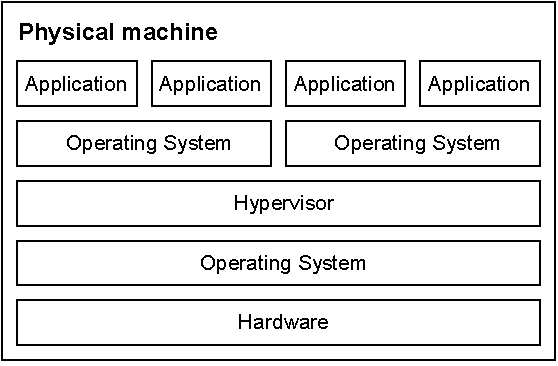
\includegraphics[width=0.65\textwidth]{Figures/virtualization.pdf}
	\caption{Brief presentation of the virtualization technology\cite{RamosApolinario.2021, Warrier.20201120}. Multiple \acp{OS} run on the same physical machine simultaneously. The hardware is mocked by the hypervisor layer.}
	\label{fig:background.virtualization}
\end{figure}

Besides isolating the \ac{OS} kernel and all of its processes, the network layer also has to be isolated. This is usually achieved by three  different approaches:
\begin{itemize}
\item \textbf{Network address translation} One approach is to convert the network packets between the \ac{VM} and the host computer based on \ac{NAT}. This means, the host computer provides a network interface which is connected to the \ac{VM}. Incoming and outgoing traffic to the \ac{VM} is translated using the additional virtual network interface. % TODO: Beleg
\item \textbf{Bridged network} In this approach the traffic between \ac{VM} and host computer is "bridged". This means, the \ac{VM} gets its own \ac{IP} address assigned and is seen and acts as its own member.
\item \textbf{Host network} The host network approach hides the \ac{VM} from the outer network and only allows communication between the \ac{VM} and the host machine.
\end{itemize}


Microsoft offers with \enquote{Hyper-V} its own virtualization software since \enquote{Windows 8}. % TODO: Beleg


\subsection{Container}
As shown in \autoref{fig:background.container}, Container have a more lightweight concept of isolation compared to virtualization. Instead of providing an isolation layer for both, the \ac{OS} kernel and the running processes, only the processes are isolated (\enquote{process isolation}). Compared to virtualization, this increases performance of the isolated processes and reduces the startup time.

\begin{figure}[b]
	\centering
	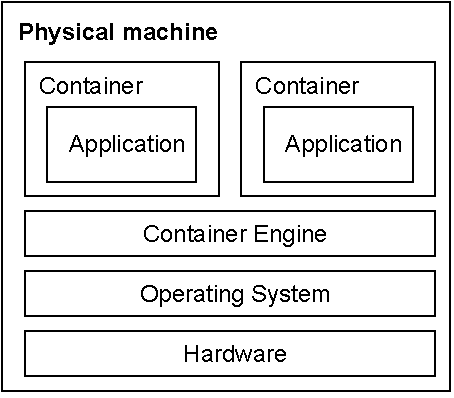
\includegraphics[width=0.5\textwidth]{Figures/containerization.pdf}
	\caption{Brief presentation of the containerization technology\cite{RamosApolinario.2021, Warrier.20201120}. Each isolated process runs inside a container, the \ac{OS} kernel is shared.}
	\label{fig:background.container}
\end{figure}

Containers share the \ac{OS} kernel with the host system.  Thus, \ac{OS} kernel and processes running inside the container have to match.
However, this does allow libraries to be shared within containers where necessary\cite{Warrier.20201120}.
The process isolation is performed by encapsulating the file system, the users, the kernel processes and the network interfaces of the host system towards the container. Each container receives its own set of those encapsulated core objects. For the isolation of the network the same strategies as for virtualization apply.

Because of their lightweight nature, containers usually only encapsulate a single application process. For encapsulating an application, one has to build a \enquote{container image}.  For the description of an image, the Containerfile format\footnote{Containerfile: https://www.mankier.com/5/Containerfile} is mostly used. The preparation of an image as \enquote{infrastructure-as-code} allows to build a reproducible environment on different machines. An example of a Containerfile is given in \autoref{lst:background.containerfile}.

\begin{lstlisting}[label=lst:background.containerfile, caption={Example of a container file. A file (file.txt) is copied to a Windows Server container (to C:\textbackslash out.txt), and this file is printed during the container run using the command.}, language=docker]
FROM mcr.microsoft.com/windows/server:ltsc2022
COPY file.txt C:\out.txt
CMD type C:\out.txt
\end{lstlisting}

Container images can derive from other images that can derive from images again, and so on. Thus, an image definition consist of a general part as baseline (the \enquote{base image}) and an application specific part. On top of this chain is an image for containerizing the \ac{OS} processes. From which base image a container image derives is defined by the \tcode{FROM} statement (line~1).
The value after \tcode{FROM} defines the address to the base image, whereas the value \enquote{ltsc2022} is called \enquote{image tag} and usually used for defining a concrete version of the base image. In this case, this is \enquote{\ac{Windows} Server 2022}.

Other statements can be given, for example, for copying files into the container file system (line~2), running commands for preparing the image or defining meta data about the image. The statement \tcode{CMD} (line~3) defines the command that is automatically run and monitored, once the container image has started. If this command exits, the container is also automatically terminated.

If images are not available on a host system, they are \enquote{pulled} from a \enquote{container registry}. It is a server that hosts the images, and is available either public or private.


\section{Problem statement}
Even though, the application is clearly based on a microservice architecture and is able to run on a distributed system, it is not designed for an automated cluster yet.

Containerization of the system has never been tested and needs to be introduced. 
This is why one focus lies on the containerization of the application. Due to its complexity with \ac{mTLS} encrypted communication and its sophisticated behavior with spawning new processes on demand, the containerization on \ac{Windows} based system is challenging.
Moreover, virtualization on \ac{Windows} has shifted more and more towards containerization in recent years. Nevertheless, true process isolation is still a rather rarely used technology under Windows. This circumstance makes research and development of \ac{Windows} containers quite challenging and therefore containerization of the application must be investigated first.

As prerequisite, the application needs to be adapted. Error handling and logging is not present in the current application. 
Even though the front end application does write logs, the microservices currently do not produce log files. Instead, only a few sub processes write the information on its standard output stream. In some cases, the error information given by exceptions is dropped.
Furthermore, proper exit codes in error cases are not returned. That is, if the application exits there is currently no way to detect if the process terminated normally or crashed as part of an error.
Therefore, for simplifying development of the container image logging must be introduced and proper error handling should be optimized.


The second focus lies on the setup of the cluster with regards to \ac{Windows} nodes.
First, the cluster engine needs to be set up. Since clustering with \ac{Windows} containers is uncommon, preliminary studies where \ac{Windows} nodes are part of a cluster are rare. Some cluster designs should be probed to provide a qualitative statement about which configuration is feasible.
After adding the \ac{Windows} node to the cluster, the network interface has to be set up to provide connectivity between the services and nodes. 
The created containerized application must be provided to the cluster engine so that it can be rolled out. Thus, automatic deployment of the developed images in the cluster engine has to be investigated. 
The functional connectivity of the services has to be ensured by checking the connectivity with regards to the \ac{mTLS} encryption.


\section{Limitations}
Due to the limited amount of time, not all code changes are applied. On the one hand, this involves the adaption for automatic extension of services. On the other hand, it implies the changes required to make the application more fault-tolerant. The changes that would be necessary, would be too extensive. Therefore, they are only made to the main processes.

This thesis aims to provide a proof of concept for shifting an existing application to the cluster. Since the previous research in the field of host-process container applications is rather limited, the focus is on the investigation of using \ac{Windows} nodes as part of the cluster.
This is why the application is not fully containerized. As part of this study, only the main services are containerized and the cluster is set up to investigate the behavior in cluster environments. 
Instead of offering a complete step-by-step guide, challenges during the development of the deployment automation are found.
 
% !TeX spellcheck = en_US
\chapter{System design} % Main chapter title

\label{chap:design} % Change X to a consecutive number; for referencing this chapter elsewhere, use \ref{ChapterX}

\lhead{Chapter \ref*{chap:design}. \emph{System design}} % Change X to a consecutive number; this is for the header on each page - perhaps a shortened title
Various applications for realizing the architecture have been compared. In the following sections the different options that were taken into account are presented.

\section{Orchestration engine}
Orchestration engines aggregate the processes and tools that are used to distribute services across multiple machines. Further, multiple replications are provided to maintain reliability. In addition, some solutions offer load balancing of incoming requests and network interconnection.
What all of these engines have in common is that a group of virtual machines or containers, known as \enquote{nodes}, are managed from a central spot. An administrator directs what application is run on the cluster. Based on the application's metadata, the orchestration engine then decides where to run the application by selecting a node inside that cluster.

\subsection{Hyper-V Replication} Microsoft \ac{Windows} supports a replication mechanism for virtual machines hosted by Hyper-V. The existing virtual machines are mirrored to secondary virtual machine host servers which highers scalability and reliability. Therefore, by replicating to a secondary Hyper-V host server, enabling process continuity and recovery on outages is ensured.
Although there are benefits, like scalability and recovery, Hyper-V is mainly designed for virtual machines. Therefore, the cluster management solution is not applicable for this use case.

\subsection{Docker Swarm} \enquote{Docker Swarm} is a cluster and orchestration engine for the container service \enquote{Docker}. The offered extension mode has more features compared to the Hyper-V replication and is specialized for containers. For example, Load Balancing, increased fault tolerance and automatic service discovery.
A highlighted feature among Docker Swarm is the decentralized design. That means, manager and application service can both run on any node within the cluster. Since it comes with Docker, no additional installation is required if Docker is already installed on the system.
However, since it is bound to the Docker \ac{API}, using this orchestration technology involves the risk of inflexibility later on (\enquote{vendor lock-in}).

%\paragraph{Open Shift}
%"Open Shift" is a application platform for clustering and orchestration of containers. It encapsulates \ac{K8s} and is similar to Kubernetes. It is also not free to use.
 
% andere sind mit Funktionsumfang sehr limitiert?
\subsection{Kubernetes}
\acf{K8s} is a orchestration engine similar to \enquote{Docker Swarm}. Load balancing, auto-scaling and automatic service discovery are also offered. However, \ac{K8s} additionally comes with the ability to rollback to a previous version in a product life cycle and has built-in support for auto-scaling.
However, \ac{K8s} has more sophisticated configuration options which makes it harder to configure in the beginning.


The engine of choice was \ac{K8s} because of its rich feature set.
Also studies showed that \ac{K8s} outperforms Docker Swarms when it comes to performance. For example, Marathe et.~al.~\cite{Marathe.2019} compared a simple web server service deployed on a Docker Swarm cluster with a \ac{K8s} cluster. The results showed better performance for \ac{K8s} in terms of memory consumption and CPU usage. Another study of Kang~et.~al.~\cite{Kang.2021} compared the performance of Docker Swarm and \ac{K8s} in a limited computing environment on Raspberry Pi boards. They also concluded that \ac{K8s} outperforms Docker Swarm if used with a high amount~(=30) of service containers on 3~Pi boards~\cite{Kang.2021}. Since they focused on container distribution and management methods this might get handy in the use case scenario under study.


\section{Kubernetes}
Since \ac{K8s} is the chosen orchestration engine, the following sections are taking a deeper look inside its architecture.

\subsection{Entities}
There are many entities for objects inside the cluster. For description of those entities the configuration language YAML\footnote{YAML: https://yaml.org/} is used. Some of the most widely used entities are described in the following paragraphs.

\paragraph*{Pod} A pod represents a set of running containers on a node. Each pod has additional information stored, such as Health state, the cluster internal network \ac{IP} address or the amount of replications.
\paragraph*{Deployment}
Deployments are used to define declarative states for Pods. This allows to maintain consecutive versions of the pod and upgrade them during runtime.
\paragraph*{Daemon set} These ensure that multiple (or all) nodes run a certain pod\cite{Kubernetes.20220831}. Common use cases are tasks for all nodes or running the network overlay pod.
\paragraph*{Configuration Map} A configuration map stores non-confidential data as key-value pair\cite{Kubernetes.20221024b}. Data stored in a configuration map can be mounted as volume, environment variable or command line argument to make applications more portable\cite{Kubernetes.20221024b}.
\paragraph*{User} This entity describes a user that  can access the \ac{K8s} cluster and \ac{API} services. Users can be part of a group and permission roles.
\paragraph*{Node} A node represents a physical machine inside the cluster. Nodes can run multiple pods.


\subsection{Services}
\ac{K8s} comes with a set of core services (see \autoref{fig.kubernetes-architecture}) that ensure the life span of scheduled containers, and the compute services that offer the actual application.
\begin{figure}[h]
	\centering
	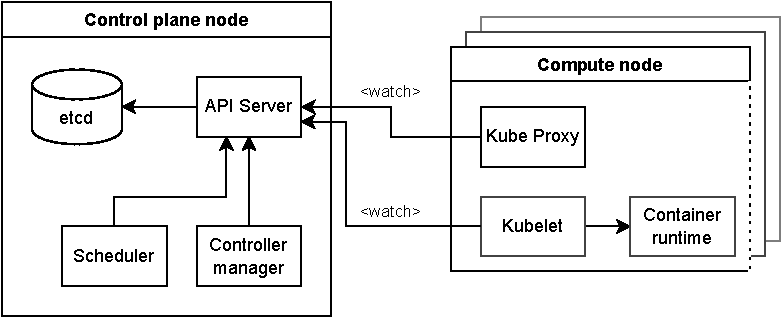
\includegraphics[width=.95\textwidth]{Figures/kubernetes-architecture.pdf}
	\caption{Core and compute services for Kubernetes\cite{Luksa.2018}}
	\label{fig.kubernetes-architecture}
\end{figure}

In the following paragraphs, the crucial services are described in detail. Since every service is a pod, they can have multiple replicas. Only the core service have to run on a dedicated Linux node the so called \enquote{control plane node} or \enquote{master node}. The underlying \ac{OS} must be Linux, because \ac{Windows} is not supported as control plane. The other services can run on nodes (with any \ac{OS}) for executing the applications and perform computations (\enquote{compute node} or \enquote{worker node}).

The services are controlled by the \ac{CLI} tools \enquote{kubectl} and \enquote{kubeadm}. While \enquote{kubectl} controls the deployment of services and application on the cluster, \enquote{kubeadm} is for setting up the cluster initially.
Furthermore, the tool \enquote{crictl} can be separately installed for the inspection of the local \ac{CRI} on a node. It allows insights into the  containers and images, but also into locally installed pods. Additionally, pods and containers can be managed using this tool.

\paragraph*{etcd}
The etcd\footnote{etcd: https://etcd.io/} database server is a key-value store designed for distributed systems\cite{Luksa.2018}. That means it could run with multiple replications and would still be able to keep a persistent storage synchronized across multiple instances. It contains the applied configuration of several cluster entities (e.g. User configurations, deployments, pod configurations).

\paragraph*{API server}
This is a RESTful web server that serves the Kubernetes \ac{API} via \ac{HTTP}\cite{Kubernetes.20221024}. It is the central joint between the services and establishes communication between users, external components and other core services. It makes the objects stored in etcd accessible over an Open \ac{API} specification\cite{Luksa.2018,OpenAPIInitiative.20230210} and allows observing changes on the entities. The \ac{CLI} tools \enquote{kubectl} and \enquote{kubeadm} both interact with the \ac{API} server.

\paragraph*{Kubelet} Kubelet is the service on the \ac{OS} level that maintains the pod life cycle and ensures the runtime of a container inside a pod. Furthermore, it manages the registration of the node to the control plane and reports its health and pod status to the \ac{API} server.

\paragraph*{Kube Proxy} The Kube-Proxy runs as a separate pod on every compute node. It maintains the connectivity between the services and pods\cite{Luksa.2018}. For a given \ac{IP} address and port combination it assures the connection to the corresponding pod. If multiple pods can offer a service, the proxy also acts as a load balancer\cite{Luksa.2018}.

\paragraph*{Scheduler} The scheduler is responsible for distributing services on the cluster and determining which node to choose during runtime. It reads conditions for scheduling (e.g. hardware resources, \ac{OS}, labels) from the \ac{API} server and decides which node matches the configuration\cite{Luksa.2018}.

\paragraph*{Controller manager} While the \ac{API}-Server is responsible for storing data in etcd and announcing changes to the clients, the Controller manager and its parts try to achieve a described target state\cite{Luksa.2018}. The controller manager consists of several controllers for replications, daemon sets, deployments, volumes, and so on.


\subsection{Pod life cycle}
\label{chap:design.life_cycle}
Similar to the underlying application container, Pods in \ac{K8s} have a ephemeral lifetime\cite{Kubernetes.20230217}. After creation on the cluster, a unique identifier is assigned before a pod gets scheduled to an available node\cite{Kubernetes.20230217}. The pod keeps alive until its termination or deletion\cite{Kubernetes.20230217}.
For distinguishing different kind of states of a pod life cycle, \ac{K8s} defines the pod states as described in \autoref{tbl:k8s-pod-states}.

\begin{table}[h!]
	\centering
	\begin{tabular}{|l | p{.65\textwidth}|} 
		\hline
		\bfseries State & \bfseries Description  \rule{-5pt}{2.6ex} \\
		\hline \rule{-3pt}{3ex}
		Pending & The pod has been set up, the container and pod is currently initialized. \\
		\hline
		Running & The pod is bound to a node, the container is running. \\
		\hline
		Succeeded & The container terminated with a zero exit code. \\ 
		\hline
		Failed & The container terminated with a non-zero exit code or was terminated by the system. \\ 
		\hline
		Unknown & The pod state could not be obtained. \\ 
		[1ex] 
		\hline
	\end{tabular}
	\caption{List of \ac{K8s} states during pod life cycle\cite{Kubernetes.20230217}.}
	\label{tbl:k8s-pod-states}
\end{table}

A terminated pod automatically gets restarted based on a configured restart policy. As the \ac{K8s} documentation states, \enquote{the kubelet restarts them [the containers of a pod] with an exponential back-off delay (10s, 20s, 40s, …), that is capped at five minutes}\cite{Kubernetes.20230217}. Furthermore, it is explained that the back-off time gets reset, once a container keeps running for 10 minutes\cite{Kubernetes.20230217}.


\subsection{Cluster networking}
Cluster networking is achieved using two components: The network plugin and the \ac{CNI}. Pods receive their own \ac{IP} address and can communicate with other pods. However, this is not a functionality which is achieved by \ac{K8s} directly. By using a \ac{CNI} the automated generation of network addresses and their inclusion is achieved when new containers are create or destroyed. It is crucial that pods share the same subnet across all the nodes in a cluster and \ac{NAT} is avoided\cite{Luksa.2018}.

Network plugins do implement the \ac{CNI}. They usually come with a manifest for a daemon set that introduces a network agent on all nodes inside the cluster to support the network communication.
For setting up the network interface, namespace and its \ac{IP} address, a dedicated container image is used. This is called the \enquote{pause container} image.

\paragraph*{Flannel}
Flannel\footnote{Flannel: https://github.com/flannel-io/flannel} was originally developed as part from Fedora CoreOS\footnote{CoreOS: https://getfedora.org/en/coreos}\cite{SuseRancherCommunity.20230212}. It works with various backends for transferring packets in the internal network. Two possible backends are virtual extensible Local Area Network (\enquote{vxlan}) and host gateway (\enquote{host-gw}). While \enquote{host-gw} needs an existing infrastructure and performs routing on the layer 3 network level, VXLAN is more flexible and could also be used in cloud environments\cite{GitHubFlannel.io.20230212}. As shown in \autoref{fig:design.flannel-network}, VXLAN is an overlay protocol and encapsulates layer 2 Ethernet frames within datagrams\cite{SuseRancherCommunity.20230212}. It is similar to regular VLAN and offers more than 4,096 network identifiers\cite{SuseRancherCommunity.20230212}. Thus, VXLAN is a good choice for highly scalable systems.

\begin{figure}[h]
	\centering
	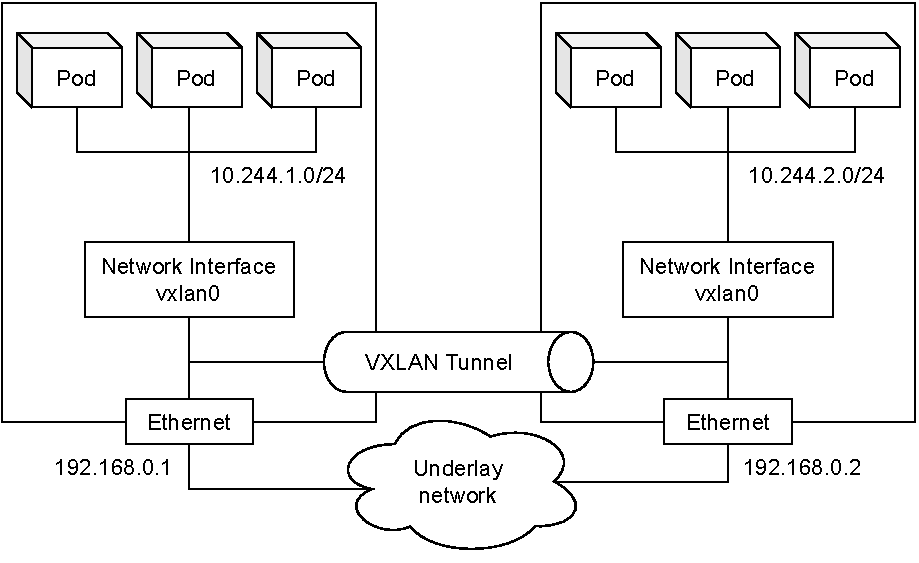
\includegraphics[width=.95\textwidth]{Figures/flannel-network.pdf}
	\caption{Flannel overlay network architecture for \ac{K8s}\cite{Schott.2019}. The pods have their own \ac{IP} address range and traffic gets routed through a VXLAN tunnel.}
	\label{fig:design.flannel-network}
\end{figure}

Even though, the team behind \ac{K8s} do not recommend any specific network plugin, there are only a few common network plugins widely used. The amount of available \ac{CNI} plugins is even more reduced if the support for \ac{Windows} nodes is taken into account.

\paragraph*{Calico}
Compared to Flannel, Calico\footnote{Tigera's Calico: https://www.tigera.io/project-calico/} is stated to be more performative, flexible and powerful\cite{SuseRancherCommunity.20230212,Tigera.20230210}. Calico comes with a sophisticated access control system\cite{Tigera.20230210} and more configuration options. However, its advanced configuration makes it hard to maintain long-term.

For this use case, Flannel is used as network plugin, since it is the described plugin used in the documentations for setting up \ac{K8s} with \ac{Windows} containers\cite{GitHubKubernetesSIGWindowsTools.20230213,Kubernetes.20220419}. Hence, support for this \ac{CNI} plugin in relation with \ac{Windows} containers is assumed to be larger than with Calico.




\section{Container environment}
The ecosystem around containerization defines terminology that needs to be looked at before going into details for \ac{K8s}. First of all, the \acf{CRI} defines the interface between \ac{K8s} and container runtime. Most of the container runtimes follow the design principles defined by the Open Container Initiative (OCI)\footnote{OCI: https://opencontainers.org/} for describing images and containers. The actual container runtime runs the isolation layer between the physical host machine and the \ac{K8s} cluster by using containerization of processes. This is what can be selected when working with \ac{K8s}.

While \ac{K8s} used to support Docker as their standard container runtime, they announced it to be deprecated in 2020, and finally removed the support in February 2022\cite{Kubernetes.2020, Kubernetes.2022}. The teams behind \ac{K8s} decided to drop the hard coded support for Docker and offer ContainerD instead.
However, the specification for ContainerD's \enquote{Containerfile} has only minor differences compared to Docker's \enquote{Dockerfile}. Thus, ContainerD files are fully compatible to docker files.

Some of the container runtimes offered by \ac{K8s} are not available for \ac{Windows} hosts. For example, Linux containers (LXC)\footnote{LXC: https://linuxcontainers.org/} use process groups, \acp{cgroup} and name spaces on the \ac{OS} level.
The \ac{CRI} from the Open Container Initiative (CRI-O)\footnote{CRI-O: https://cri-o.io/} is another alternative offered for \ac{K8s} on Linux systems. Since those are not available in \ac{Windows}, they are not further considered.

At the current time being, container networking with ContainerD is not well-established on \ac{Windows}~\cite{GitHub.20230202,GitHub.20230202b,Github.2022_258,GitHub.20230202c} even though the docker runtime is already removed in current versions of \ac{K8s}~\cite{Kubernetes.2020}. However, these are the only two working container backends for \ac{Windows} containers. Therefore ContainerD as container backend was chosen.

\subsection{ContainerD}
ContainerD is a native version of a container runtime. Newer versions of Docker on Linux, are running ContainerD under the hood for process isolation. On \ac{Windows}, ContainerD uses slim host process isolation.  The process isolation with ContainerD consists of multiple abstraction layers (shown in \autoref{fig.containerd-architecture}). Its back end contacts the containerd-shim which is maintaining an abstraction layer for communication for the underlying layers (depending on Linux and \ac{Windows}). Below that, \ac{Windows} offers a custom fork of the \ac{CLI} \textit{runc}, so called \textit{runhcs}\cite{Scooley.2022}. Using \textit{runc}, new containers can be created by running a simple command\cite{Scooley.2022}. The layer for \textit{runhcs} connects to the \ac{HCS} which is another abstraction layer of \ac{Windows} for providing a stable \ac{API} to the low level functionality of the \ac{OS}\cite{Microsoft.2017}. ContainerD does not come with any mechanisms for networking. Instead, this is in responsibility of the \ac{HCS}.

The developers of \ac{K8s} marked the Docker \ac{CRI} as deprecated in version v1.20\cite{Kubernetes.2020}. Since version v1.23 of \ac{K8s}, Docker was fully removed which lead to ContainerD being the only available \ac{CRI} for \ac{Windows} containers.

\begin{figure}[hb]
	\centering
	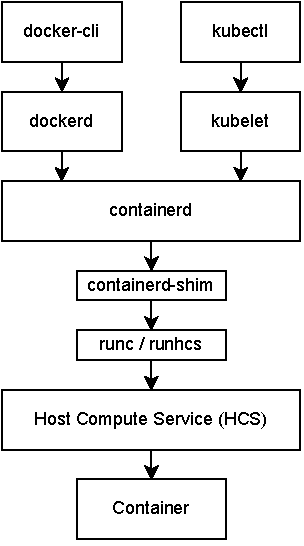
\includegraphics[width=0.4\textwidth]{Figures/containerd-architecture.pdf}
	\caption{Abstraction layers for ContainerD on Windows. The image shows the technology stack from the Docker and \ac{K8s} command line to the Container layer.\cite{Scooley.2022}}
	\label{fig.containerd-architecture}
\end{figure}

% TODO: CLI tools for ContainerD
There are two \ac{CLI} tools that work with ContainerD. The tool \enquote{ctr} is the low level \ac{CLI} tool that is shipped with ContainerD.  \enquote{nerdctl} is a tool that is similar to the Docker \ac{CLI}  and supports the same set of commands and options as Docker. Compared to \enquote{ctr}, however, \enquote{nerdctl} is more feature-rich.


\subsection{Docker Container Runtime Interface}
The Docker \ac{CRI} (so called \enquote{Docker shim}) is using the internal mechanisms from Docker to run containers. Older versions in Linux were using control group isolation.

For \ac{Windows}, there are two different isolation modes available. The first option is using the process isolation (so called \enquote{Host process isolation}) mode offered by ContainerD. It can be enabled by switching to \enquote{\ac{Windows} Containers}. It is the default mode for Windows Server systems.
However, older versions of Docker and Docker on Windows 10 and above have the opposite behavior\cite{RamosApolinario.2021}. On client versions of Windows, a dedicated hypervisor-isolated virtualization (so called \enquote{Hyper-V isolation}) is the default option\cite{RamosApolinario.2021}. This means, during the installation of Docker on \ac{Windows}, the underlying Windows container host creates a separate Hyper-V \ac{VM} to run container images. However, this is not a regular Hyper-V \ac{VM}\cite{RamosApolinario.2021}. Instead, it is a purpose-built \ac{VM}, often referred to as utility \ac{VM} or UVM that can't be managed directly and is fully controlled by the \ac{Windows} container runtime\cite{RamosApolinario.2021}. For networking, the internal mechanisms from Docker are used. All running containers are deployed inside the dedicated Hyper-V \ac{VM}. Therefore, this is a mixture of process isolation and full isolation using virtualization.

However, the hypervisor approach still has the disadvantage of using large resources for containers, even though they are running in one virtual machine. In addition, containers running in hypervisor isolation take longer to start up than those running in process isolation\cite{RamosApolinario.2021}.




\section{Container Image}
There are container images for each process of the system architecture, each of them having their own Containerfile definition with different command line arguments and environment variables.
The container image and its base image is further explained in this section.

\subsection{Base image}
The container images to use for running the OpenTwin processes need to run a \ac{Windows} base image. Beside the full \ac{Windows} images, Microsoft offers the more common images \enquote{\ac{Windows} Server Core} and \enquote{\ac{Windows} Nanoserver}\cite{MattbriggsMicrosoft.20230214}. They significantly differ in the download size, their on-disk footprint and the features supported\cite{MattbriggsMicrosoft.20230214}. As Microsoft states, \enquote{Nanoserver was built to provide just enough \ac{API} surface to run apps that have a dependency on .NET core or other modern open source frameworks. PowerShell, Windows Management Instrumentation, and the \ac{Windows} servicing stack are absent from the Nanoserver image}\cite{MattbriggsMicrosoft.20230214}.

The design of containerization of \ac{OT} envisages the usage of \enquote{Server Core} as base image. Even though the \enquote{Server Core} image is not the smallest base image, it provides full functionality for the required technologies for the current use case.

% Warum dieses \ac{Windows} image?
% \ac{Windows} Server Core and Nanoserver are the most common base images to target. The key difference between these images is that Nanoserver has a significantly smaller \ac{API} surface. PowerShell, WMI, and the \ac{Windows} servicing stack are absent from the Nanoserver image.
% Nanoserver was built to provide just enough \ac{API} surface to run apps that have a dependency on .NET core or other modern open source frameworks. As a tradeoff to the smaller \ac{API} surface, the Nanoserver image has a significantly smaller on-disk footprint than the rest of the \ac{Windows} base images. Keep in mind that you can always add layers on top of Nano Server as you see fit. For an example of this check out the .NET Core Nano Server Dockerfile.
% Quelle: https://learn.microsoft.com/en-us/virtualization/\ac{Windows}containers/manage-containers/container-base-images

\subsection{Custom image}
On top of the base image, customizations and the actual application are applied. The binary files are included in the container image and added during build. The common \acp{CRI} only forward the output of processes with process id 1 to the host machine. Furthermore, this is also the only process the  \ac{CRI} is waiting for, to keep the container alive. Thus, instead of using the provided batch files to start the application services, the OpenTwin process is called directly with the appropriate command line arguments as command for the container.
Therefore, the environment variables needs to be set up as part of the container file.
The root certificate (certificate authority) is passed as file mount into the container later on.


\section{Target architecture}
The application is distributed on multiple systems. \ac{K8s} supports application rollouts only as container images. To be able to distribute the services on a cluster management tool a containerization of the application is necessary.
Each service shall be served on the cluster to profit from the features which \ac{K8s} offers. For example, it must be possible to offer multiple replications of services - with the compute services included. This is the only way to ensure that the application can be delivered reliably. 
However, for testing the feasibility it is sufficient to deploy only the main services as a first step. This involves \ac{GSS}, \ac{LSS} and \ac{AUTH}. Subsequently, the \ac{LSS} spawns the compute services as sub processes inside the same container. In order to communicate with the \ac{UI} front end, the connection between the external network and the relay service has to be ensured.

The MongoDB server is not required to run on \ac{Windows}. Because setting it up on Linux is easier and better supported, a dedicated Linux node for running the MongoDB server is preferred. Furthermore, automation for a MongoDB container image on \ac{Windows} is currently unsupported, because of an design limitation in Windows containers\cite{GitHub.20230317}. The \ac{OT} services, however, have to run on \ac{Windows} and are therefore deployed on a \ac{Windows} node.

The encrypted communication between services has to be ensured. As a consequence, the certificates need to be accessible for each service. The certificate files shall be published on the container file system using file mounts. This increases flexibility because files can be easily swapped out, and generated for each service outside the container. Certificate files then have to be created during pod creation.
However, as a first step, the certificates are generated as part of the image build process to keep the automation simpler.



 
\chapter{Implementation} % Main chapter title

\label{chap:implementation} % Change X to a consecutive number; for referencing this chapter elsewhere, use \ref{ChapterX}

\lhead{Chapter \ref*{chap:implementation}. \emph{Implementation}} % Change X to a consecutive number; this is for the header on each page - perhaps a shortened title

% \begin{lstlisting}[label={lst:swapoff}, caption={Bash commands for turning off swapping in Linux Debian}]
% \end{lstlisting}

\section{Containerization of Services}
Container images are provided for running the application inside the \ac{CRI}. Definition of the container manifest is done in the \enquote{Containerfile}\footnote{Containerfile: https://www.mankier.com/5/Containerfile} format.

% TODO: ENTWEDER-ODER: Build has to be done inside the container. / All binary files are part of the container image.

\subsection{Code changes on core application}
For containerizing the \ac{OT} application, several changes were applied to its code base. This improves error handling and error tracing of the application and therefore simplifies development of the cluster. In the following sections, the several code changes are described in detail.

\subsubsection*{Introduction of exit codes}
The microservice \ac{DLL} files have return codes for different error cases. This is, for instance a code 200 in the \ac{AUTH} for connection issues to the database. As with process exit codes, a zero return code indicates a successful termination. Even though the main executable \enquote{open\_twin.exe} retrieves the return code, it did not convert these codes into proper process exit codes. 
Exit-Codes are a crucial part of the \ac{K8s}'s life cycle management as described in \autoref{chap:design.life_cycle}. Therefore, the return codes need to be converted into process exit codes.

\begin{lstlisting}[label=lst:code_changes.exitcodes.before, caption={Former code snippet from main executable for calling the microservice library code in Rust (\textit{/Microservices/OpenTwin/src/main.rs})}, language=rust, firstnumber=85]
let _result = initialize(siteid_c_str.as_ptr(), service_c_str.as_ptr(), db_c_str.as_ptr(), dir_c_str.as_ptr());
\end{lstlisting}
The surrounding lines of code in the main executable are shown in \autoref{lst:code_changes.exitcodes.before}. It calls the initialization method of the microservice \ac{DLL}, passes all its parameters and retrieves its return code.

\begin{lstlisting}[label=lst:code_changes.exitcodes.after, caption={Code changes in Rust main executable for additional treatment of exit codes (\textit{/Microservices/OpenTwin/src/main.rs})}, language=rust, firstnumber=86]
if _result != 0 {
  eprintln!("Library/Service initialization ({}:init()) failed with exit code {}", lib_path, _result);
  std::process::exit(_result);
}
\end{lstlisting}
A new condition for non-zero exit codes was added as shown in \autoref{lst:code_changes.exitcodes.after}. The variable \tcode{\_result}  contains the returned exit code of the library \ac{DLL}, whereas \tcode{lib\_path} contains the path to the library \ac{DLL}. As can be seen, it is used to describe the affected service name in a error message (line 87).
 
\subsubsection*{Debug verbosity in launcher}
By default Rust programs show a window for console output no matter if it was built in release mode or with debug parameters. However, the main executable uses conditional compilation to set configuration attributes about the windows subsystem.
\begin{lstlisting}[label=lst:cond_compilation_windows_subsystem, caption={Conditional compilation for disabling console output in non-debug builds (\textit{/Microservices/OpenTwin/src/main.rs})}, language=rust, firstnumber=2]
#![cfg_attr(not(debug_assertions), windows_subsystem = "windows")]
\end{lstlisting}
Rust provides a compilation option \tcode{debug\_assertions} that is set to \enquote{true} for compilations without code optimization\cite{Rust.20230209}. Therefore it is set to \enquote{true} if the application runs in debug mode. As shown in \autoref{lst:cond_compilation_windows_subsystem} with conditional compilation, this build option is checked and console output is only shown for debug builds. If the windows subsystem is set to \tcode{windows}, no console windows are rendered after starting the application.

Even if output is shown on the console window for debug builds only, the error messages are not able to be read conveniently in cases where the application crashes. This impedes debugging and diagnosis of regular application errors outside of a containerized environment.
To avoid this behavior, the launcher batch files were adapted. For this, a new parameter was invented to the batch file for running the batch file in verbose mode.
\begin{lstlisting}[label=lst:launcher_extension.parameter_validation.after, caption={Additional command argument for preventing close of window after termination (\textit{/Microservices/Launcher/OpenTwin\_session.bat})}, language=cmd, firstnumber=18]
IF "%~1"=="/V" (
  REM OT is opening console windows in debug build, so we want to pause them at the end
  SET pause_prefix=cmd.exe /S /C "
  SET pause_suffix=" ^& pause
  ECHO ON
)
\end{lstlisting}
As first step, a new command line argument has been introduced. If \enquote{/V} is appended to the start of the launcher batch file it will run with higher verbosity.  As can be seen in \autoref{lst:launcher_extension.parameter_validation.after}, with \enquote{/V} appended, two new variables \tcode{pause\_prefix} and \tcode{pause\_suffix} are set (line 20-21). Furthermore, command output is enabled to debug the launcher file itself (line 22).

\begin{lstlisting}[label=lst:launcher_extension.call.after, caption={Additional command extension for preventing close of window after termination (\textit{/Microservices/Launcher/OpenTwin\_session.bat})}, language=cmd, firstnumber=34]
START "AUTHORIZATION SERVICE" %pause_prefix%open_twin.exe AuthorisationService.dll <*@ \Suppressnumber @*>
  "%OPEN_TWIN_SERVICES_ADDRESS%:%OPEN_TWIN_AUTH_PORT%" "%OPEN_TWIN_MONGODB_ADDRESS%"
  "%OPEN_TWIN_MONGODB_PWD%"%pause_suffix% <*@ \Reactivatenumber @*>
\end{lstlisting}
The newly defined variables \tcode{pause\_prefix} and \tcode{pause\_suffix} are then appended to the command of starting a service. This is shown in \autoref{lst:launcher_extension.call.after}. It ensures that a service process is started in a new window and the command is followed by the \ac{Windows} \enquote{pause} command to stop and wait for user interaction. Thus, the user is now able to read error messages if application crashes occur.

\subsubsection*{Enhanced logging and error tracing}
For improving the error tracing, the overall log amount has been increased. This involves enabling the logging of the central logging functions inside the library \enquote{OpenTwinCommunication}. The logging mechanism did not use logging to standard output. Instead, calls to the respective functions for logs were just ignored. This was changed and logging to standard output has been introduced. 
\begin{lstlisting}[label=lst:implementation.log_message_filter, caption={Comparison of the set log level with the log severity of the message. If the converted log severity is less than the defined log level, the message is ignored. (\textit{/Libraries/OpenTwinCommunication/src/ServiceLogger.cpp})}, language=c++, firstnumber=60]
if (((int)_severity) < ((int)m_logLevel)) {
	return;
}
\end{lstlisting}
Log messages also have information stored about their severity that can be converted from \enquote{enum} values to their numeric representation. With respect of the high amount of printed log messages, they are now filtered by their severity. This filter mechanism is shown in \autoref{lst:implementation.log_message_filter}.

Additionally, more calls to the logging mechanism, including caller information, have been added. For instance, the \ac{AUTH} now shows error messages for caught exceptions and errors during database initialization.
Also, the general error tracing has been improved. In the main services \ac{GSS}, \ac{LSS} and \ac{AUTH}, exception handling has been added, where it was not present before. Furthermore, the formatting of exception messages was improved and more information has been added.

For the current time being, there is an ongoing work to replace the logging to standard output by forwarding the log lines to a central logging library.

\subsubsection*{Certificate changes}
Since \ac{OT} is using \ac{mTLS} for communication between services, the \ac{CSR} file needs to contain the host specification for the outgoing \ac{IP} address and host name. Thus, in \ac{OT} a batch script substitutes placeholders in a template \ac{CSR} file. The respective section of the \ac{CSR} template is shown in \autoref{lst:implementation.mtls_csr_replacement}.
\begin{lstlisting}[label=lst:implementation.mtls_csr_replacement, caption={Variables defined in the \ac{CSR} are substituted by their respective values. (\textit{/Deployment/Certificates/server-csr\_template.json})}, language={}, firstnumber=3]
  "hosts": ["$HOSTNAME$", "$IP_ADDRESS$", "localhost", "127.0.0.1"],
\end{lstlisting}
However, this process does not work if performed for a containerized application. If the replacement takes place during the creation of the container, the final host name or \ac{IP} address does not yet exist. If, on the other hand, the automatic replacement is done later, it cannot be carried out from outside the container, as the script automatically replaces only the local host name.
To solve this problem, the \ac{CSR} template was extended by fixed values for \enquote{localhost} and \enquote{127.0.0.1}. This already covers the majority of use cases. Additionally, it is recommended to not generate the certificate as part of the container image build process. Instead it should be inserted via a file mount.

\subsubsection*{Listening on all interfaces}
Container images have a certain network image for communicating to external hosts. Processes inside the container have to bind to this network interface. However, the \ac{IP} address of this network interface is unpredictable during compile time. The processes that run inside a container therefore have to bind to all available network interfaces to be accessible to the outer network which is performed by binding on the address \enquote{0.0.0.0}.
Moreover, the services exchange service information with other services as described in \autoref{chap:background.baseline_architecture}. Because the binding address \enquote{0.0.0.0} is invalid and not accessible from the public, it must differ from this published address in a containerized environment.

Instead of binding to all network interfaces, the main executable in \ac{OT} was only able to bind to a given \ac{IP} address (based on the published service address) only. Also, it was not possible to configure a different binding address than the one published to other services.

\begin{lstlisting}[label=lst:listen_all_interfaces.before, caption={Listener binding before the applied changes (\textit{Microservices/OpenTwin/src/main.rs})}, language=rust, firstnumber=145, numbers=left]
let listener = net::TcpListener::bind(&service_url).await?;
println!("Starting server at {:?}", service_url);
\end{lstlisting}
\autoref{lst:listen_all_interfaces.before} shows the affected lines of code in the main executable. The passed argument for the service \ac{URL} is forwarded to the server listener class. Afterwards, the address is printed on the console. The service \ac{URL}, here passed as variable, consists of the service address and the port of the service.

To not affect the outer interface, the changes work with the data already provided. This means, the passed arguments to the main executable are not altered.
\vspace{4em}
\begin{lstlisting}[label=lst:listen_all_interfaces.after, caption={Listener binding after the applied changes. The service url is parsed, based on its port. Binding is done on all interfaces. (\textit{Microservices/OpenTwin/src/main.rs})}, language=rust, firstnumber=150]
let service_port = Url::parse(&format!("https://{}", service_url))
.expect(&format!("Invalid service url. Unable to parse service url: {}", service_url))
.port();
if service_port.is_none() {
	panic!("Invalid service url. Service url is lacking port defintion: {}", service_url);
}
let binding_address = format!("0.0.0.0:{}", service_port.unwrap().to_string());
let listener = net::TcpListener::bind(&binding_address).await?;
println!("Server listening on {:?} (publishing {:?})", binding_address, service_url);
\end{lstlisting}
The binding address is separated from the published address, since the address in the argument still gets passed to the microservice \ac{DLL}. Afterwards, the service \ac{URL} is processed as shown in \autoref{lst:listen_all_interfaces.after}. First, the given service \ac{URL} is parsed and the port number is extracted (lines 150-152). If no port is found or the parsing failed, the application fails and shows an error (lines 153-155). Afterwards, the port number is concatenated with the binding address \enquote{0.0.0.0} and therefore the server binds to all addresses (lines 156-157). The last line shows the new output containing the port number and the address published to other services.

% TODO - Bugfix for OpenGL error in uiFrontend (not necessary??)

\subsection{Container definition}
There were three container images prepared for containerization of \ac{OT}. These cover the main services for \ac{GSS}, \ac{LSS} and \ac{AUTH}. The structure is the same for each of the container files. The first part of the container file is shown in \autoref{lst:containerfile.1}.
\begin{lstlisting}[label=lst:containerfile.1, caption={Containerfile for the \ac{LSS}. Description of the base image and variable tagging using a build argument. (\textit{Distribution/Container/session.Containerfile})}, language=docker, firstnumber=1]
ARG BASE_IMAGE_TAG=ltsc2022
FROM mcr.microsoft.com/windows/servercore:$BASE_IMAGE_TAG
\end{lstlisting}
The first line introduces a build argument for defining the target image tag from the command line without altering the container file.  It is used afterwards to pass the image tag to the base container image. The subsequent lines define labels for the resulting image.
\vspace{1em}
\begin{lstlisting}[label=lst:containerfile.3, caption={Containerfile for the \ac{GSS}. Description of the command line and certificate creation. (\textit{Distribution/Container/session.Containerfile})}, language=docker, firstnumber=21]
ENTRYPOINT ["cmd", "/C"]
CMD ["open_twin.exe", "SessionService.dll", "0", \
"%OPEN_TWIN_LSS_SERVICE_ADDRESS%:%OPEN_TWIN_LSS_PORT%", \
"%OPEN_TWIN_GSS_SERVICE_ADDRESS%:%OPEN_TWIN_GSS_PORT%", \
"%OPEN_TWIN_AUTH_PORT%"]
EXPOSE 8093
WORKDIR C:/app/Deployment/Certificates
COPY ./ ../
RUN createCertificate.bat && certutil -addstore root %OPEN_TWIN_CA_CERT%
WORKDIR C:/app/Deployment
RUN C:\app\Deployment\VC_Redist\VC_redist.x64.exe /install /quiet
\end{lstlisting}
\autoref{lst:containerfile.3} shows the lower section of the container file for containerizing the \ac{LSS}.
The container files differ in the runtime specification. They run the same entry point, but have a different process running as command. Besides, the exposed port depends on the service inside the container. 
After defining the command and copying the files into the container image (lines 22-28), the certificates are built as part of the image file system (line 29). Since the compute services are dependent to C++ libraries that are not present in the base image, the Microsoft Visual C++ Redistributable must be installed as well (line 31).

% Container image must be built on each node machine manually. Since the Windows base image os is only compatible with the respective host operating system.
% Deployment-Verzeichnis muss dafür initial auf Node kopiert werden.
% TODO: (Skript ("setup-node") dafür schreiben, was neusten release von github zieht (RUN download?) und image autom. baut + image pusht?)  - base image (FROM) mittels args dynamisch gestalten?


\section{Cluster Setup}
The following section describes the setup of different nodes in the cluster. While the master node refers to the \ac{K8s} control plane node which is responsible for distribution of the workers, the worker nodes are the actual machines that are executing the applications.
The used version of \ac{K8s} is \enquote{v1.25.3}. The version of ContainerD is \enquote{v1.6.8}, on both sides, the worker nodes and the master node.

\subsection{Setting up the master node}
For setting up the master node on Linux, a system based on Debian Bullseye 11.5 was used. Basis for the performed steps is the \ac{K8s} documentation for setting up a container runtime\cite{Kubernetes.2019} and the online tutorial of Basappa\cite{Basappa.2022}.

\subsubsection{Installing prerequisites and ContainerD}
After installing and setting up the operating system, the swap mechanism needs to be permanently turned off. This is done by editing the file system table (\tcode{fstab}), in file \tcode{/etc/fstab} respectively, by commenting out the swap partitions and masking the systemd swap units as shown in \autoref{lst:disable_swap}.
\begin{lstlisting}[label=lst:disable_swap, caption={Bash commands for disabling Swap mechanism and masking.}, language=bash]
$ sed -i '/ swap / s/^\(.*\)$/#\1/g' /etc/fstab
$ systemctl mask dev-sda3.swap
\end{lstlisting}

The container runtime requires certain kernel features to be enabled. On Debian 11, the required kernel modules for virtual networking facilities (\tcode{br\_netfilter}) and overlay filesystems (\tcode{overlay}) are not enabled by default. Thus, they have to be manually enabled.
% To permanently enable them and keep them enabled after reboot, the setting is stored in a file as shown in \autoref{lst:kernel_modules}.
To permanently enable them and keep them enabled across reboots, the setting is stored in a file in the directory for loaded modules (\textit{/etc/modules-load.d/k8s.conf}).
\begin{comment}
% https://www.natarajmb.com/2022/06/kubernetes-debian/
\begin{lstlisting}[label=lst:kernel_modules, caption={Bash commands for enabling required kernel modules.}, language=bash]
$ cat <<EOF | sudo tee /etc/modules-load.d/k8s.conf 
overlay 
br_netfilter 
EOF 
\end{lstlisting}
\end{comment}

For functional networking on the master node, \ac{K8s} also requires internal network packets being forwarded to the pods. Additionally, the tracking table for tracing network packets and their assigned connection is increased. This is a prerequisite for the applied \ac{NAT} which is used in container networking.
New files with respective settings are created in the directory for kernel settings as shown in \autoref{lst:ip_forward}.
\begin{lstlisting}[label=lst:ip_forward, caption={Bash commands for enabling \ac{IP} forwarding and network filtering.}, language=bash]
$ cat <<EOF | tee /etc/sysctl.d/k8s.conf 
  net.bridge.bridge-nf-call-iptables  = 1
  net.bridge.bridge-nf-call-ip6tables = 1
  net.ipv4.ip_forward                 = 1 
  net.netfilter.nf_conntrack_max      = 524288 
EOF
$ echo 1 > /proc/sys/net/ipv4/ip_forward
\end{lstlisting}

After installing ContainerD with all its prerequisites from the package registry, a configuration file (\tcode{config.toml}) is created.
Subsequently, the SystemD \ac{cgroup} is added to the runtime options of ContainerD and its service is restarted. For this, the commands from \autoref{lst:master.containerd_config} are applied.
\vspace{1em}
\begin{lstlisting}[label=lst:master.containerd_config, caption={Bash command for setting up containerd config},language=bash, morekeywords={sudo, kubeadm, tee, service}]
$ containerd config default | <*@ \Suppressnumber @*>
  sed 's/\[plugins.\"io.containerd.grpc.v1.cri\".containerd.runtimes.runc.options\]/&\n SystemdCgroup = true/' | tee /etc/containerd/config.toml >/dev/null <*@ \Reactivatenumber @*>
$ service containerd restart
\end{lstlisting}

To finally start the cluster, the packages for the Kubelet service, \enquote{kubeadm} and \enquote{kubectl} need to be installed. Then, the cluster can be initialized by running the command line tool as shown in \autoref{lst:master.kubeadm.init}. Since the configuration parameters can also be passed as YAML file, this is the preferred method of passing arguments and allows version control of the required configuration.
\begin{lstlisting}[label=lst:master.kubeadm.init, caption={Bash command for setting up the cluster}, morekeywords={sudo, kubeadm}, numbers=none]
$ kubeadm init --config kubeadm_config.yaml
\end{lstlisting}

Since Flannel is used as network overlay, the \ac{IP} address range provided for pods must be \enquote{10.244.0.0/16}\cite{GitHubKubernetesSIGWindowsTools.20230213}. Additionally, a value is provided that sets the \ac{CRI} socket address for newly registered nodes to the one of ContainerD. Furthermore, the \ac{cgroup} driver for the Kubelet service on worker nodes is set to SystemD. Thus, the \ac{cgroup} driver on Linux worker nodes should be aligned to the master node.
The information passed as configuration is presented in \autoref{lst:master.kubeadm.config}.
\begin{lstlisting}[label=lst:master.kubeadm.config, caption={YAML configuration for providing configuration for the cluster and newly registered ndoes. (\textit{Distribution/Controlplane/kubeadm\_config.yaml})}, language=yaml]
kind: ClusterConfiguration
apiVersion: kubeadm.k8s.io/v1beta3
kubernetesVersion: v1.25.3
networking:
  podSubnet: "10.244.0.0/16" # pod-network-cidr
---
kind: InitConfiguration
apiVersion: kubeadm.k8s.io/v1beta3
nodeRegistration:
  criSocket: unix:///var/run/containerd/containerd.sock
---
kind: KubeletConfiguration
apiVersion: kubelet.config.k8s.io/v1beta1
cgroupDriver: systemd
\end{lstlisting}


\subsubsection{Applying a Container Network Interface}
After successfully initializing the cluster, the overlay network for Flannel must be set up.
For this, the respective entity description can be directly downloaded from the vendor\footnote{Flannel entity description: \href{https://raw.githubusercontent.com/flannel-io/flannel/master/Documentation/kube-flannel.yml}{https://raw.githubusercontent.com/flannel-io/flannel/master/Documentation/kube-flannel.yml}}. Since networking has to blend with Flannel on \ac{Windows}, the \ac{VNI} (4096) and port (4789) for Flannel on \ac{Windows} must be set as part of the configuration. For this, manual editing of the description must be performed. The respective values are added to the configuration map section where the network configuration file is described (the section \enquote{net-conf.json} of \enquote{kube-flannel.yml}) as shown in \autoref{lst:implementation.flannel_fixup}. This file is automatically created on newly registered nodes. The changed entity description is applied on the cluster respectively.
\begin{lstlisting}[label=lst:implementation.flannel_fixup, caption={Fixup for Flannel manifest. Here the values \tcode{VNI} and \tcode{Port} were added. (\textit{kube-flannel.yml})}]
net-conf.json: | {
  "Network": "10.244.0.0/16",
  "Backend": {
    "Type": "vxlan",
    "VNI" : 4096,
    "Port": 4789
}}
\end{lstlisting}
\vspace{-2em}
\subsubsection{Adding the proxy daemon sets}\vspace{-1em}
The usage of \ac{Windows} worker nodes in a \ac{K8s} cluster requires additional configuration mappings and daemon sets to be applied on the cluster. Those are used for setting up a proxy for Flannel. The \ac{SIG} \enquote{Windows Tools} of \ac{K8s} provides the additional objects\cite{GitHubKubernetesSIGWindowsTools.20230213}. Before applying them, a replacement of the \ac{K8s} version and the Flannel version is performed. This procedure is achieved by running the two commands shown in \autoref{lst:master.proxy_daemonsets}. 
\begin{lstlisting}[label=lst:master.proxy_daemonsets, caption={Bash command for adding the flannel overlay configuration\cite{GitHubKubernetesSIGWindowsTools.20230213}}, language=bash]
$ curl -L https://raw.githubusercontent.com/kubernetes-sigs/sig-windows-tools/master \<*@ \Suppressnumber @*>
  /hostprocess/flannel/kube-proxy/kube-proxy.yml | 
  sed 's/KUBE_PROXY_VERSION/v1.25.3/g' | 
  kubectl apply -f -<*@ \Reactivatenumber @*>
$ curl -L https://raw.githubusercontent.com/kubernetes-sigs/sig-windows-tools/master \<*@ \Suppressnumber @*>
  /hostprocess/flannel/flanneld/flannel-overlay.yml | 
  sed 's/FLANNEL_VERSION/v0.17.0/g' | 
  kubectl apply -f -<*@ \Reactivatenumber @*>
\end{lstlisting}


\subsection{Setting up the worker node}\label{chap:implementation.setup_worker}
The initialization of the worker node is mainly oriented on the guide for adding \ac{Windows} nodes that is provided from the \ac{SIG} \enquote{Windows Tools} on GitHub\cite{GitHubKubernetesSIGWindowsTools.20230213}. Although there is an original guide from \ac{K8s}\cite{Kubernetes.20220419}, it was not used as basis because it is outdated.

First, the node preparation scripts of the \ac{K8s} \ac{SIG} \enquote{Windows Tools} are retrieved and executed as shown in \autoref{lst:worker.sig_scripts}. The first script retrieved (\textit{Install-Containerd.ps1}) installs ContainerD and its prerequisites on \ac{Windows}. Installation of the prerequisites involves the Windows features \enquote{Hyper-V}, \enquote{Hyper-V Tools}, \enquote{Hyper-V for PowerShell} and \enquote{Containers}. Once the features are installed and the system has successfully rebooted, the script has to be restarted. It then proceeds by downloading the binary of ContainerD and adding its location to the \tcode{PATH} environment variable. ContainerD's configuration file is changed to align the \ac{CNI} file locations with \ac{K8s}. The script ends by registering ContainerD as a service.

The second script (\textit{PrepareNode.ps1}) prepares the node for joining the cluster. It first downloads the Kubelet executable and creates a script file that is called by the Kubelet service. The created script file contains runs the Kubelet in consideration of version dependent command arguments. Afterwards, the \ac{NSSM}\footnote{NSSM: https://nssm.cc/} is downloaded and the Kubelet script is registered as a service. Finally, the \textit{PrepareNode} script also sets up firewall rules for Kubelet.

Furthermore the command line tools \enquote{kubectl}, \enquote{kubeadm}, \enquote{crictl} and \enquote{nerdctl} are installed. While installing \enquote{crictl}, it is added to the \tcode{PATH} environment variable.

\begin{lstlisting}[label=lst:worker.sig_scripts, caption={Retrieval of node preparation scripts\cite{GitHubKubernetesSIGWindowsTools.20230213}}, language=PowerShell, morekeywords={curl.exe, Install-Containerd.ps1, PrepareNode.ps1}]
> curl.exe -LO https://raw.githubusercontent.com/kubernetes-sigs/sig-windows-tools/master/kubeadm/scripts/Install-Containerd.ps1
> .\<*@\textbf{Install-Containerd.ps1}@*>
> curl.exe -LO https://raw.githubusercontent.com/kubernetes-sigs/sig-windows-tools/master/kubeadm/scripts/Prepare<*@\kern.7pt@*>Node.ps1
> .\PrepareNode.ps1 -KubernetesVersion v1.25.3
\end{lstlisting}

% \begin{comment}
%service.
%% [plugins."io.containerd.grpc.v1.cri"].sandbox_image
%For having a valid image at a later point in time, the \ac{CRI} value \tcode{sandbox\_image} in ContainerD's configuration file (\textit{config.toml}) needs to be replaced with a newer version.
%
%After successfully setting up the \ac{NAT} and installing ContainerD as a service, the node will be finally prepared to host tasks. For this, another Powershell script \enquote{PrepareNode}\footnote{https://github.com/kubernetes-sigs/sig-windows-tools/releases/download/v0.1.5/PrepareNode.ps1} from the Kubernetes \ac{SIG} runs. After running the script, the resulting \enquote{StartKubelet} file needs to be changed to drop invalid arguments.
%
%% C:\k\kubelet.exe $global:KubeletArgs --cert-dir=$env:SYSTEMDRIVE\var\lib\kubelet\pki --config=/var/lib/kubelet/config.yaml --bootstrap-kubeconfig=/etc/kubernetes/bootstrap-kubelet.conf --kubeconfig=/etc/kubernetes/kubelet.conf --hostname-override=$(hostname)
%Furthermore, the following lines were added to the Kubelet configuration:
%\begin{lstlisting}[label=lst:master.configtoml_changes, caption={Configuration changes in ContainerD configuration file (\textit{config.toml})\cite{GitHubKubernetesSIGWindowsTools.20230213}}]
%enforceNodeAllocatable: []
%cgroupsPerQOS: false
%enableDebuggingHandlers: true
%\end{lstlisting}
%These configuration values are valid for \ac{Windows} machines only and cause an error in Kubelet on Linux. The configuration changes therefore can only be served to Windows machines and the configuration on the nodes needs to be changed locally.
%\end{comment}


% Es wurde "New-HnsNetwork -Type NAT -Name nat -Gateway 10.244.0.1 -AdressPrefix 10.244.240.0/20" ausgeführt
% TODO: Evtl. testen, ob man mit Docker auf Netzwerk zugreifen kann? "Object already exists"
% TODO: -- siehe: https://github.com/kubernetes-sigs/sig-windows-tools/issues/128

After successfully running the preparation script the node should be ready to join the cluster. For joining the cluster a token is generated on the master node. The token is copied to the preapared node and used as part of a \enquote{join} command. \autoref{lst:worker.join} shows the command for joining the cluster, whereas the token is substituted by \enquote{TOKEN}.
\begin{lstlisting}[label=lst:worker.join, caption={Command for joining new nodes on Windows}, language=PowerShell, morekeywords={kubeadm.exe}]
> kubeadm.exe join 1.2.3.4:6443 --token TOKEN --discovery-token-ca-cert-hash sha256:HASH \<*@ \Suppressnumber @*>
  --cri-socket "npipe:////./pipe/containerd-containerd"<*@ \Reactivatenumber @*>
\end{lstlisting}
Besides containing the token and the master node's \ac{IP} address, the command also has the hash value of the \ac{CA} of the master node. For \ac{K8s} versions \enquote{v1.25} and below the command also requires the explicit declaration of ContainerD as container runtime. Thus, the additional option \tcode{cri-socket} is defined.

The successful join of the node is verified by running \tcode{kubectl get nodes} on the master node. This prints the newly added node.

\subsection{Deployment of the application}
As a first draft, only the \ac{LSS} of the application is deployed. 
Deployment of the application is done by applying the manifest as shown in \autoref{lst:deploy.yaml}.
The manifest defines a pod using the container image of the \ac{LSS} (lines 2-4). Since the images are not yet provided via an image registry, the images are stored locally. Thus, the \ac{K8s} is directed to never pull the image and retrieve it locally instead.
The passed environment variables (lines 5-13) are defined by the section \tcode{env}, whereas the variable \tcode{OPEN\_TWIN\_LSS\_SERVICE\_ADDRESS} is set with the \ac{IP} address of the pod. The external port is defined as 8093, which is equivalent to the port of the \ac{LSS}.
The node selector property (lines 16-17) defines a requirement for the node scheduler to select only \ac{Windows} nodes.
The manifest is applied on the cluster using \tcode{kubectl apply}.
\begin{lstlisting}[label=lst:deploy.yaml, caption={Partial section of configuration for cluster deployment of the \ac{LSS} (\textit{Distribution/Kubernetes/open\_twin.yaml})}, language=yaml]
containers:
- name: opentwin-session
  image: local.dev/opentwin-session:latest
  imagePullPolicy: Never
  env:
    - name: OPEN_TWIN_LSS_SERVICE_ADDRESS
      valueFrom:
        fieldRef:
          fieldPath: status.podIP
    - name: OPEN_TWIN_MONGODB_ADDRESS
      value: 1.2.3.4:27017
    - name: OPEN_TWIN_GSS_SERVICE_ADDRESS
      value: 5.6.7.8
  ports:
  - containerPort: 8093
nodeSelector:
  kubernetes.io/os: windows
\end{lstlisting}


\section{Automatic setup}
% TODO: Powershell script beschreiben
Even though the scripts provided from the \ac{SIG} \enquote{Windows Tools} cover most of the preparation steps, some manual steps are still required as described in the respective guide\cite{GitHubKubernetesSIGWindowsTools.20230213}. To automate the preparation process where possible, and to also provide tools for debugging error cases, further steps are required. Thus, a custom script (\textit{Distribution/Container/setup-node.ps1}) was created to provide this aid.

The script automates the process of rebooting and rerunning the preparation after the required \ac{Windows} features are installed, and provides instructions for steps that cannot be automated. It also checks the prerequisites before performing any action. This means, it is checked whether the operating system is \enquote{\ac{Windows} Server} and if a certain minimum version of \ac{Windows} is used. The check for prerequisites is shown in \autoref{lst:auto.check_preq}.
\begin{lstlisting}[label=lst:auto.check_preq, caption={Powershell commands in the automated setup script. Checks for prerequisites.}, language=PowerShell]
if (-not ((Get-ComputerInfo).WindowsProductName | Select-String "Server")) {
  throw "Prerequisites not met. Windows Server is required as operating system."
}
if (-not (Get-Hotfix -ErrorAction Ignore KB4489899)) {
  if (-not ([System.Environment]::OSVersion.Version -gt [System.Version]"10.0.17763.0")) {
    throw "Prerequisites not met. You either need KB4489899 installed, or a Windows Version higher than 10.0.17763"
  }
}
\end{lstlisting}

Besides checking for system requirements, the custom script also installs tools for debugging. This includes the \ac{Windows} version of \enquote{kubeadm} and \enquote{kubectl}, as well as the command line tools for debugging containers on \ac{Windows}, namely \enquote{crictl} and \enquote{nerdctl}.
Furthermore, the custom script also excludes the ContainerD process from the \ac{Windows} Defender firewall as shown in \autoref{lst:auto.win_defender}. This increases the pull and general runtime performance of containers.
The installation of the command line tools also involves setting up PowerShell auto completion and include to the \tcode{PATH} environment variable.
\begin{lstlisting}[label=lst:auto.win_defender, caption={Powershell command in the automated setup script. Exclusion of all actions performed by containerd.exe from Windows Defender.}, language=PowerShell, numbers=none]
Add-MpPreference -ExclusionProcess "$Env:ProgramFiles\containerd\containerd.exe"
\end{lstlisting}


 
\chapter{Discussion} % Main chapter title

\label{chap:discussion} % Change X to a consecutive number; for referencing this chapter elsewhere, use \ref{ChapterX}

\lhead{Chapter \ref*{chap:discussion}. \emph{Discussion}} % Change X to a consecutive number; this is for the header on each page - perhaps a shortened title


\section{Analysis}

\section{Dunno whata write yet...}
% !TeX spellcheck = en_US
\chapter{Conclusion and future work} % Main chapter title

\label{chap:conclusion} % Change X to a consecutive number; for referencing this chapter elsewhere, use \ref{ChapterX}

\lhead{Chapter \ref*{chap:conclusion}. \emph{Conclusion and future work}} % Change X to a consecutive number; this is for the header on each page - perhaps a shortened title


\section{Lessons learned}
% man kann sich hier auch wiederholen; für leute, damit sie nicht nochmal die gleichen fehler machen-

\section{Conclusion}

\section{Future work}
- Linux  port and cluster based on linux
- Automated image building using Packer.io (for multiple platforms)
- Ranger for streamlining kubernetes deployment
- Images verkleinern - nur die Dateien ins Image bundlen, die für den entsprechenden Service notwendig sind.
- Put certificate files into container via file mount - Design?

- Falls OT sowieso in Container gebaut werden muss, dann kann dieser Schritt auch automatisiert werden (clone aus git, bauen mit Build Tools)
- Dann ist auch nicht mehr nötig, Deployment Verzeichnis manuell auf jeden Node zu kopieren.


- Blockzitat: K8s checkliste, zur korrekten Funktionsweise des Netwerks -> Funktioniert nicht

- GPU einbinden für compute services?

 

%----------------------------------------------------------------------------------------
%	THESIS CONTENT - APPENDICES
%----------------------------------------------------------------------------------------

\addtocontents{toc}{\vspace{2em}} % Add a gap in the Contents, for aesthetics

\appendix % Cue to tell LaTeX that the following 'chapters' are Appendices

% Include the appendices of the thesis as separate files from the Appendices folder
% Uncomment the lines as you write the Appendices

% Appendix A

\chapter{Appendix Title Here} % Main appendix title

\label{AppendixA} % For referencing this appendix elsewhere, use \ref{AppendixA}

\lhead{Appendix A. \emph{Appendix Title Here}} % This is for the header on each page - perhaps a shortened title

Write your Appendix content here.
%\input{Appendices/AppendixB}
%\input{Appendices/AppendixC}

\addtocontents{toc}{\vspace{2em}} % Add a gap in the Contents, for aesthetics

\backmatter


%----------------------------------------------------------------------------------------
%	ACRONYMS
%----------------------------------------------------------------------------------------

\label{acronyms}
\lhead{\emph{Acronyms}}
\begin{acronym}[cgroup]
\acro{OT}{OpenTwin}
	
\acro{Windows}{Microsoft\textsuperscript{\tiny\textregistered} Windows\textsuperscript{\tiny\textregistered}}	
	
\acro{cgroup}[cgroup]{control group}
\acro{SIG}[SIG]{Special Interest Group}
\acro{DLL}[DLL]{Dynamic Link Library}{Dynamic Link Libraries}
\acro{URL}{Uniform Resource Locator}
\acro{UI}{User Interface}

\acro{TLS}{Transfer Layer Security}
\acro{mTLS}{mutual Transfer Layer Security}

\acro{GSS}{Global Session Service}
\acro{AUTH}{Authorization Service}
\acro{LSS}{Local Session Service}

\acro{HTTP}{Hypertext transfer protocol}
\acro{API}{Application Programming Interface}
\acro{CLI}{Command line interface}

\acro{K8s}{Kubernetes}
\acro{IP}{Internet Protocol}
\acro{NAT}{Network Address Translation}
\acro{CNI}{Container Network Interface}
\acro{CRI}{Container Runtime Interface}


\acro{VM}{Virtual Machine}
\acro{HCS}{Host Compute Service}

\end{acronym}

%----------------------------------------------------------------------------------------
%	BIBLIOGRAPHY
%----------------------------------------------------------------------------------------

\label{Bibliography}

\lhead{\emph{Bibliography}} % Change the page header to say "Bibliography"

\bibliographystyle{unsrtnat} % Use the "unsrtnat" BibTeX style for formatting the Bibliography

\bibliography{Bibliography} % The references (bibliography) information are stored in the file named "Bibliography.bib"

\end{document}  